\documentclass[11pt]{extarticle}

\usepackage[a4paper,top=2cm,bottom=2cm,left=3cm,right=3cm,marginparwidth=1.75cm]{geometry}
\usepackage{blindtext}
\usepackage{listings}
\usepackage{titlesec}
\usepackage[utf8]{inputenc}
\usepackage[greek,english]{babel}
\usepackage{alphabeta}
\usepackage{float}
\usepackage{rotating}
\usepackage{lscape}
\usepackage{tabu}
\usepackage{indentfirst}
\usepackage[perpage]{footmisc}
\usepackage{multicol}
\usepackage{xcolor,colortbl}
\definecolor{lgray}{rgb}{0.8, 0.8, 0.8}
\usepackage{caption}
\captionsetup[table]{name=Πίνακας}
\captionsetup[figure]{name=Διάγραμμα}
\usepackage{fancyhdr}
\usepackage[
    backend=bibtex,
    style=alphabetic,
    sorting=ynt
    ]{biblatex}
\addbibresource{refs.bib}

\definecolor{codegreen}{rgb}{0,0.6,0}
\definecolor{codegray}{rgb}{0.5,0.5,0.5}
\definecolor{codepurple}{rgb}{0.12,0.12,0.12}
\definecolor{backcolour}{rgb}{1, 1, 1}
\lstdefinestyle{mystyle}{
    backgroundcolor=\color{backcolour},   
    commentstyle=\color{codegray},
    keywordstyle=\color{codepurple},
    numberstyle=\tiny\color{codegray},
    stringstyle=\color{codepurple},
    basicstyle=\ttfamily\scriptsize,
    breakatwhitespace=false,         
    breaklines=true,                 
    captionpos=b,                    
    keepspaces=true,                 
    numbers=left,                    
    numbersep=5pt,                  
    showspaces=false,                
    showstringspaces=false,
    showtabs=false,                  
    tabsize=4
}
\lstset{style=mystyle}

\titleformat{\section}[display]{\huge\sc}{Κεφάλαιο \thesection}{0pt}{\large}

\pagestyle{fancy}
\rhead{\thepage}
\lhead{\rightorleftmark}
\cfoot{}

\makeatletter
\newcommand{\rightorleftmark}{%
  \begingroup\protected@edef\x{\rightmark}%
  \ifx\x\@empty
    \endgroup\nouppercase\leftmark
  \else
    \endgroup\rightmark
  \fi}
\makeatother


\usepackage{amsmath}
\usepackage{graphicx}
\usepackage{svg}
\usepackage[colorlinks=true, allcolors=blue, unicode]{hyperref}
\usepackage[perpage]{footmisc}
\renewcommand{\thefootnote}{\fnsymbol{footnote}}
\renewcommand{\footnotesize}{\fontsize{11pt}{13pt}\selectfont}

\let\stdsection\section
\renewcommand\section{\newpage\stdsection}

\newcommand{\instbit}[1]{\mbox{\scriptsize #1}}
\newcommand{\instbitrange}[2]{~\instbit{#1} \hfill \instbit{#2}~}
\newcommand{\reglabel}[1]{\hfill {\tt #1}\hfill\ }

\title{Μια ενδεικτική υλοποίηση RISC-V επεξεργαστή και ενός υποστηρικτικού Assembler}
\author{Λασκαρέλιας Βάιος}



\begin{document}
\begin{titlepage}
    \begin{center}
        \vspace*{1cm}

        \makebox[\textwidth][c]{
            \centering
            
\includegraphics[width=0.6\textwidth]{diagrams/logo.pdf}
        }
        \newline

        {\Large Πολυτεχνική Σχολή\\
        Τμήμα Μηχανικών Η/Υ \textampersand\space Πληροφορικής\par}
        \vspace*{0.8cm}
        {\LARGE Διπλωματική Εργασία\par }
        \makebox[\textwidth][c]{
            \centering
            \rule{\textwidth}{0.4pt} }
        \hfill \newline
        \vspace*{0.3cm}
        \textbf{\Huge Μια ενδεικτική υλοποίηση RISC-V επεξεργαστή και ενός υποστηρικτικού Assembler} \par

        \vspace{0.5cm}

        {\huge UPatras RISC-V} \par
        \vspace*{0.3cm}
        \makebox[\textwidth][c]{
            \centering
            \rule{\textwidth}{0.4pt} }
        \hfill \newline
        \vspace{1cm}

        \textbf{\LARGE Βάιος Λασκαρέλιας}\par
        \vspace*{0.2cm}
        {\Large A.M.: 1054432} \par
        \vspace*{1.5cm}
        \Large
        Επιβλέπων\\\vspace*{0.2cm}
        Χαρίδημος Βέργος, Καθηγητής\\
        \vspace*{0.8cm}
        Μέλη Εξεταστικής Επιτροπής\\\vspace*{0.2cm}
        Δημήτριος Νικολός, Καθηγητής\\
        Νικόλαος Σκλάβος, Αναπληρωτής Καθηγητής\\
        \vfill
             
        Πάτρα, Οκτώβριος 2021
             
    \end{center}
 \end{titlepage}
% \maketitle
\newpage

\renewcommand{\abstractname}{Ευχαριστίες}\begin{abstract}\normalsize
    Θα ήθελα να εκφράσω την εκτίμησή μου για τους ανθρώπους που με στήριξαν έμπρακτα σε όλη την πορεία των σπουδών μου.
    Χωρίς αυτούς, η εκπόνηση αυτής της διπλωματικής εργασίας δεν θα ήταν δυνατή.
\end{abstract}
\nopagebreak
\hfill \newline
\makebox[\textwidth][c]{
    \centering
\rule{\textwidth}{0.4pt} }
\hfill \newline
\renewcommand{\abstractname}{Thanks}\begin{abstract}\normalsize
    I would like to express my appreciation to each and every one who supported me during my studies.
    Without them, the completion of this thesis would not be possible.
\end{abstract}
\newpage

\renewcommand{\abstractname}{Περίληψη}\begin{abstract}\normalsize
Η παρούσα διπλωματική εργασία υλοποιεί ένα λειτουργικό θεωρητικό μοντέλο ενός διασωληνωμένου επεξεργαστή βασισμένου στην αρχιτεκτονική RISC-V, υλοποιημένο σε Icarus Verilog, με έμφαση στην απλότητα της τελικής σχεδίασης.
Το μοντέλο συνοδεύεται από έναν συμβατό, επεκτάσιμο Assembler για την διευκόλυνση του προγραμματισμού του επεξεργαστή, γραμμένο σε C, με την βοήθεια των εργαλείων Flex και Bison.
Ο Assembler είναι συμβατός με οποιονδήποτε επεξεργαστή βασισμένο στην αρχιτεκτονική RV32I.

Για την επιβεβαίωση της σωστής και κατά των προδιαγραφών λειτουργίας του μοντέλου, εκτελέστηκε μεγάλος αριθμός πιθανών ακραίων περιπτώσεων μεμονωμένων εντολών και ακολουθιών εντολών.
Τα παραγόμενα αποτελέσματα των εντολών συγκρίθηκαν με αυτά που περιγράφονται στις προδιαγραφές κατά την διάρκεια, και μετά το τέλος της εκτέλεσής τους.
Για τον έλεγχο του Assembler, παρήχθησαν περίπλοκα διανύσματα εντολών και κωδικοποιήσεων άμεσων δεδομένων, τα οποία ελέγθηκαν χειροκίνητα και διασταυρώθηκαν με άλλους συμβατούς RISC-V Assembler.
Τελικά, ο Assembler παράγει τα ορθά διανύσματα κωδικοποιήσεων των εντολών και το μοντέλο του επεξεργαστή εκτελεί τα προγράμματα με τα αναμενόμενα αποτελέσματα, κάνοντας το σύνολο των υλοποιήσεων συμβατό με την αρχιτεκτονική RISC-V.
\end{abstract}
\nopagebreak
\hfill \newline
\makebox[\textwidth][c]{
    \centering
\rule{\textwidth}{0.4pt} }
\hfill \newline
\renewcommand{\abstractname}{Abstract}\begin{abstract}\normalsize
The processor is a timeless concept of Computer Science, since it materialises the theoretical concepts of Information Theory.
Starting from the theoretical Turing Machine and the mechanical Analytical Engine of Charles Babbage, to todays chaotic Artificial Intelligence models and interconnected clusters of supercomputers, the processor is an integral piece of every computation system today. \newline

This thesis implements a working theoretical model of a RISC-V compatible CPU, implemented in Icarus Verilog, designed with simplicity in mind.
This CPU model is accompanied by a compatible, extensible RISC-V Assembler, written in C with the help of Flex and Bison tools, in order to make the model's CPU programming easier.
The Assembler is compatible with every RV32I CPU implementation.

For verification of the correctness and specification compliance of the CPU model a large number of instructions and streams of instructions was executed, covering possible edge cases.
Results of the intructions execution were observed during, and after their execution and was made sure they followed the specification's descriptions.
The assembler was checked by manually checking generated complex instruction and immediate data encodings and also comparing against other RISC-V compatible assembler implementations.
\end{abstract}
\newpage
\renewcommand{\contentsname}{Περιεχόμενα}
\tableofcontents
\renewcommand{\listfigurename}{Κατάλογος Διαγραμμάτων}
\listoffigures
\renewcommand{\listtablename}{Κατάλογος Πινάκων}
\listoftables


\section{ΕΙΣΑΓΩΓΗ}
\subsection{Περί Επεξεργαστών}
Οι επεξεργαστής είναι ένα διαχρονικό κομμάτι της επιστήμης της πληροφορικής καθώς ενσαρκώνει την πρακτική υλοποίηση της θεωρίας υπολογισμού.
Ξεκινώντας από τις θεωρητικές μηχανές Turing και την μηχανική Αναλυτική Μηχανή του Charles Babbage, μέχρι τα σημερινά χαοτικά μοντέλα τεχνητής νοημοσύνης και τα διασυνδεδεμένα συμπλέγματα υπερυπολογιστών, ο επεξεργαστής αποτελεί αναπόσπαστο μέρος κάθε υπολογιστικού συστήματος.

Η ανάγκη που οδήγησε στην δημιουργία των επεξεργαστών ξεκινάει ακόμα και πριν την επιστήμη της πληροφορικής.
Οι μαθηματικές πράξεις εκτελούνταν από ανθρώπινο δυναμικό, απαιτώντας πολύωρη επαναληπτική εργασία και οδηγώντας πολλές φορές σε λάθη.
Οι πρώτοι επεξεργαστές, πριν ακόμα οριστεί ο όρος, κατασκευάστηκαν για να εκτελούν επαναλαμβανόμενες μαθηματικές πράξεις και αλγόριθμους σε δεδομένα, παράγοντας ένα χρήσιμο μαθηματικό αποτέλεσμα \cite{forouzan}.
Ακόμα και σήμερα, η λειτουργία ενός επεξεργαστή μπορεί να περιγραφεί από την επεξεργασία δεδομένων εισόδου που παράγει ένα χρήσιμο αποτέλεσμα.
Η γενική αυτή διαδικασία της επεξεργασίας δεδομένων χρησιμοποιείται πλέον ευρέως σε κάθε τομέα της τεχνολογίας, καθιστώντας τον επεξεργαστή ένα διαχρονικό στοιχείο της επιστήμης των υπολογιστών.

\subsection{Αρχιτεκτονική Συνόλου Εντολών}
Αρχιτεκτονική συνόλου εντολών (Instruction Set Architecture - ISA) ονομάζεται ο ορισμός όλων των εντολών προς εκτέλεση από έναν επεξεργαστή, καθώς και ο ορισμός των συνεπειών από την εκτέλεση κάθε μίας από αυτές τις εντολές.
Πρόκειται δηλαδή για το μέρος του επεξεργαστή το οποίο εκτίθεται στο λογισμικό και προσφέρει έναν καλώς ορισμένο και τυποποιημένο τρόπο επικοινωνίας του υλικού με το λογισμικό \cite{patterson}.
Οι συνέπειες των εκτελέσεων των εντολών μπορούν να είναι αριθμητικά αποτελέσματα, αλλαγή της ροής του προγράμματος με βάση μια συνθήκη ή κατάσταση, αλλαγή της κατάστασης που βρίσκεται ο επεξεργαστής. 
Οι ορισμοί αυτών των εντολών συνοδεύονται από την δυαδική κωδικοποίησή τους. 
Θεωρούμε πως ένας επεξεργαστής είναι συμβατός με μία αρχιτεκτονική συνόλου εντολών, εφόσον εκτελεί την ίδια ακολουθία δυαδικών κωδικοποιήσεων εντολών έχοντας τις συνέπειες που αναφέρονται από τον ορισμό των εντολών στην αρχιτεκτονική.
\hfill\newline

Οι αρχιτεκτονικές συνόλου εντολών μπορούν να κατηγοριοποιηθούν σε δύο τύπους:
\begin{description}
\item[Αρχιτεκτονικές RISC] Reduced Instruction Set Computer
\begin{itemize}
    \item Περιορισμένος αριθμός εντολών που εκτελούν βασικές λειτουργίες γενικού σκοπού.
    \item Κάθε μία εντολή είναι ορισμένη έτσι ώστε να εκτελεί μία απλουστευμένη λειτουργία.
    \item Οι λειτουργίες επεξεργασίας δεδομένων και προσπέλασης της μνήμης δεδομένων διαχωρίζονται σε ξεχωριστές εντολές.
\end{itemize}

\item[Αρχιτεκτονικές CISC] Complex Instruction Set Computer
\begin{itemize}
    \item Μεγάλος αριθμός εντολών που είναι στοχευμένες σε λειτουργίες ειδικού σκοπού.
    \item Υπάρχει πληθώρα εντολών όπου η καθεμία από αυτές εκτελεί μια πολύ συγκεκριμένη, εξειδικευμένη λειτουργία.
    \item Μία εντολή μπορεί να κάνει ταυτόχρονα προσπέλαση της μνήμης δεδομένων και επεξεργασία δεδομένων.
\end{itemize}
\end{description}

\newpage
Ένα μεγάλο σύνολο εντολών με περίπλοκες λειτουργίες δυσκολεύει τόσο την ανάπτυξη συμβατών επεξεργαστών, αλλά και αποδοτικών compiler.
Αρχιτεκτονικές CISC, για παράδειγμα η x86, μπορεί να έχουν εντολές οι οποίες προσπελαύνουν την μνήμη μέχρι και 50 φορές κατά την εκτέλεσή τους[REF].
Οι προδιαγραφές που ορίζει μια CISC αρχιτεκτονική καθιστούν ακόμα και μια θεωρητική υλοποίηση ενός συμβατού με αυτές επεξεργαστή, πολύ πολύπλοκη.
Αυτό έχει οδηγήσει πολλούς εμπορικούς x86 επεξεργαστές να μετατρέπουν εσωτερικά την εντολή x86 σε μια ακολουθία απλούστερων εντολών παρόμοιων με αυτές των RISC αρχιτεκτονικών \cite{patterson}.
\subsection{Η αρχιτεκτονική RISC-V}
Η αρχιτεκτονική συνόλου εντολών RISC-V είναι μια RISC αρχιτεκτονική, η οποία σχεδιάστηκε στο Berkeley University of California, αρχικά από τους Andrew Waterman, Yunsup Lee, David A. Patterson, Krste Asanovic, για ακαδημαϊκούς και εκπαιδευτικούς σκοπούς \cite{spec}. 
Η σχεδιαστική της φιλοσοφία βασίζεται στην απλότητα, την παραμετροποίηση και την επεκτασιμότητα με βάση πολλά μικρά, ανεξάρτητα σύνολα εντολών.
Η ύπαρξη επεκτάσεων σε ένα βασικό σύνολο εντολών και το ευρύ πεδίο εφαρμογών δεν αποτελεί την ειδοποιό διαφορά όσον αφορά την αρχιτεκτονική RISC-V σε σχέση με άλλες, αλλά πρόκειται για τον κύριο στόχο της αρχιτεκτονικής.

Το πλεονέκτημα της αρχιτεκτονικής RISC-V βρίσκεται στο γεγονός πως σχεδιάστηκε από την αρχή για τους παραπάνω σκοπούς. 
Η παραμετροποίηση και επέκτασή της δεν αποτελεί απόρροια δημιουργίας νέων αναγκών ή ανάγκη αναπροσαρμογής μιας αρχιτεκτονικής για λύση νέων προβλημάτων. 
\subsubsection{Υλοποιήσεις RISC-V}
Ένας από τους βασικούς στόχους της αρχιτεκτονικής RISC-V είναι η αποφυγή περιορισμών με σκοπό να επιτρέψει πολλές διαφορετικές εφαρμογές τεχνικών σχεδίασης στις συμβατές υλοποιήσεις.
Η απλότητα της επιλογής των εντολών που βρίσκονται στο σύνολο καθώς και οι κωδικοποιήσεις τους, εξασφαλίζουν ευκολία όσον αφορά τις σχεδιάσεις υλικού και εξομοιωτών για ακαδημαϊκούς σκοπούς. 
Ο διαχωρισμός της αρχιτεκτονικής RISC-V σε μικρότερα προαιρετικά υποσύνολα εντολών διευκολύνει περαιτέρω την ανάπτυξη σε εκπαιδευτικά περιβάλλοντα.
Αρκετά πανεπιστήμια συμμετέχουν στο ίδρυμα RISC-V ως μέλη \cite{rvmember}.
\newline

Ακαδημαϊκές Υλοποιήσεις:
\begin{description}
    \item [BOOM (Berkeley Out-of-Order Machine)] University of California, Berkeley \cite{boom} \newline
    Παραμετροποιήσιμος συνθέσιμος (synthesizable) πυρήνας RISC-V RV64GC, με υποστήριξη Linux.
    Κύριο χαρακτηριστικό της μικροαρχιτεκτονικής του είναι η out-of-order εκτέλεση εντολών.
    \item [Riscy Processors και RiscyOO] MIT \cite{riscy}, \cite{riscyooo} \newline
    Οικογένεια RISC-V επεξεργαστών του MIT με υποστήριξη Linux.
    Βασισμένη σε προηγούμενες εργασίες των εργαστηρίων αρχιτεκτονικής του πανεπιστημίου σε MIPS Pipelined και Out-of-order επεξεργαστές.
    \item [Lizard] Cornell University \cite{lizard} \newline
    Παραμετροποιήσιμος συνθέσιμος RV64IM πυρήνας.
    Χρησιμοποιεί κατά κόρον out-of-order εκτέλεση εντολών και την τεχνική μετονομασίας Register.
    Παρέχει υποστήριξη εκτέλεσης για στατικά προγράμματα C.
\end{description}

\newpage
Η παραμετροποίηση που προσφέρει το σύνολο εντολών RISC-V καθιστά την αρχιτεκτονική κατάλληλη και για εμπορική χρήση, καθώς η χρήση των υπάρχοντων και η δημιουργία custom συμπληρωματικών υποσυνόλων εντολών (επεκτάσεων), δίνει πρακτικά απεριόριστες δυνατότητες για την κάλυψη κάθε ανάγκης.
Όπως προαναφέρθηκε, πολύπλοκες λειτουργίες που εκτελούνται από τους εμπορικά διαδεδομένους x86 επεξεργαστές ήδη μετατρέπονται σε ακολουθίες εντολών RISC, γεγονός που αποδεικνύει την ανταγωνιστικότητα που μπορεί να έχει ένας RISC-V επεξεργαστής στην αγορά. 
Κορυφαίες εταιρίες του τομέα του hardware όπως οι Google, NVidia, έχουν δείξει ενδιαφέρον για την αρχιτεκτονική συμμετέχοντας ενεργά στον οργανισμό RISC-V \cite{rvmember}.
Άξια αναφοράς αποτελεί η εταιρία SiFive, η οποία παρέχει παραμετροποιήσιμες υλοποιήσεις οικογενειών επεξεργαστών για χρήσεις γενικού σκοπού, νευρωνικών δικτύων και ενσωματωμένων συστημάτων \cite{sifive}.

Εμπορικές Υλοποιήσεις:
\begin{description}
    \item [SiFive P550] SiFive, Inc. \cite{p550}\newline
    Ο γρηγορότερος RISC-V επεξεργαστής γενικού σκοπού, με υποστήριξη Linux. 
    Βασισμένος στην αρχιτεκτονική RV64GC με out-of-order pipeline 13 σταδίων και τριπλό instruction issuing.
    \item [SweRV Core EH1] Western Digital\cite{swerv} \newline
    Ένας RV32IMC επεξεργαστής για χρήση ως ελεγκτή στα αποθηκευτικά μέσα (σκληροί δίσκοι, κάρτες μνήμης) που παράγει η εταιρία.
    Dual-issue pipeline 9 σταδίων.
    \item [NEOX Graphics] Think Silicon\cite{neox} \newline
    Οικογένεια επεξεργαστών γραφικών (GPU) βασισμένη στην αρχιτεκτονική RV64GC.
    Υποστήριξη παραμετροποίησης αριθμών πυρήνων (4-64) και την οργάνωση αυτών, multithreading, μεγέθη και οργάνωση κρυφής μνήμης.
\end{description}

\subsubsection{Σύνολο Εντολών RISC-V και Επεκτάσεις}
Το κύριο σχεδιαστικό ρεύμα της αρχιτεκτονικής RISC-V είναι ο διαχωρισμός της σε περαιτέρω μικρά υποσύνολα εντολών \cite{spec}.
Η παραπάνω σχεδιαστική νοοτροπία προσφέρει την δυνατότητα παραμετροποίησης των δυνατοτήτων του επεξεργαστή ανάλογα με τις ανάγκες της κάθε υλοποίησης.
Η ίδια η αρχιτεκτονική ενθαρρύνει την δημιουργία περαιτέρω, custom επεκτάσεων για την ικανοποίηση οποιασδήποτε ανάγκης η οποία δεν καλύπτεται από τις ήδη υπάρχουσες επεκτάσεις.
Η παραμετροποίηση επιτρέπει ελευθερία επιλογής μέχρι και στο μέγεθος του εντέλου του επεξεργαστή, δηλαδή το μήκος σε bit των αριθμών στους οποίους εφαρμόζονται οι αριθμητικές πράξεις, το οποίο αντίστοιχα ορίζει και το μήκος των διευθύνσεων της μνήμης. 

Προς το παρόν ορίζεται ένα βασικό σύνολο εντολών, το οποίο θα πρέπει να εκτελείται από κάθε επεξεργαστή αρχιτεκτονικής RISC-V, και ορισμένα στανταρισμένα υποσύνολα επεκτάσεων, για λειτουργίες που μπορεί να είναι πιθανό να φανούν χρήσιμες από πολλές υλοποιήσεις.
\begin{description}
    \item[RV32I/RV64I/RV128I] Base \newline
Το βασικό υποσύνολο εντολών \newline
Συμπεριλαμβάνει αριθμητικές και λογικές πράξεις ακεραίων, προσπελάσεις (εγγραφές και αναγνώσεις) μνήμης, εντολές διακλάδωσης και ορισμένες εντολές διαχείρισης των προσπελάσεων της μνήμης.
Κάθε μήκος εντέλου ορίζει μια διαφορετική βάση επειδή ανάλογα με το μέγεθος του εντέλου τροποποιούνται ορισμένες εντολές προσπέλασης μνήμης και εκτέλεσης πράξεων.
    \item[Επέκταση Μ] Multiplication \newline 
Πολλαπλασιασμός - Διαίρεση ακεραίων \newline
Οι πράξεις πολλαπλασιασμού και διαίρεσης έχει νόημα να οριστούν ως επέκταση καθώς απλουστεύουν την υλοποίηση μιας Αριθμητικής - Λογικής Μονάδας στις περιπτώσεις όπου δεν απαιτούνται.
    \item[Επέκταση Α] Atomics \newline
Ατομικές προσπελάσεις μνήμης \newline
Παρέχει εντολές οι οποίες χρησιμοποιούνται για την οργάνωση ατομικών προσπέλασεων κοινών μνημών μεταξύ των πυρήνων ενός RISC-V επεξεργαστή ή πολλών RISC-V επεξεργαστών.
    \item[Επέκταση F] Floating Point Arithmetic \newline
Αριθμητική κινητής υποδιαστολής \newline
Η αριθμητική κινητής υποδιαστολής ορίζεται ως επέκταση για τους ίδιους λόγους με τις πράξεις πολλαπλασιασμού - διαίρεσης.
Είναι συμβατή με την αριθμητική IEEE 754-2008.
    \item[Επέκταση D] Double Precision Floating Point Arithmetic \newline
Αριθμητική κινητής υποδιαστολής διπλής ακρίβειας \newline
Συμπληρωματική της επέκτασης F.
Προσφέρει ακριβέστερα αριθμητικά αποτελέσματα στις πράξεις αριθμών κινητής υποδιαστολής.
    \item[Επέκταση Q] Quad Precision Floating Point Arithmetic \newline 
Αριθμητική κινητής υποδιαστολής τετραπλής ακρίβειας \newline
Συμπληρωματική των επεκτάσεων F και D, προσφέρει τετραπλή ακρίβεια στις πράξεις κινητής υποδιαστολής.
    \item[Επέκταση Zicsr] Control and Status Registers \newline
Καταχωρητές ελέγχου και κατάστασης \newline
Η επέκταση ορίζει ένα σύνολο καταχωρητών κατάστασης και λειτουργίες ατομικής προσπέλασης τους.
Χρησιμοποιείται για την οργάνωση της επικοινωνίας μεταξύ πυρήνων ή επεξεργαστών, καθώς και για σκοπούς των επιπέδων του περιβάλλοντος εκτέλεσης (Machine - Hypervisor - Supervisor - User).
    \item[Επέκταση Zifencei] Instruction Fencing \newline
    Συμπληρωματική επέκταση συνέπειας μνήμης \newline
Προσθέτει εντολές για την οργάνωση των προσπελάσεων της μνήμης εντολών σε επίπεδο ενός πυρήνα RISC-V.
    \item[Επέκταση G] General Purpose \newline
    Σύνολο επεκτάσεων γενικού σκοπού \newline
Συμπεριλαμβάνει την βάση και τις επεκτάσεις M, A, F, D, Zicsr, Zifencei.
Το σύνολο εντολών που προκύπτει με τον συνδυασμό αυτών, προορίζεται για χρήση σε επεξεργαστές γενικού σκοπού, γι αυτό και στο συγκεκριμένο υποσύνολο επεκτάσεων έχει οριστεί ξεχωριστή ονομασία.
\end{description}

\section{ΤΟ ΒΑΣΙΚΟ ΣΥΝΟΛΟ ΕΝΤΟΛΩΝ RV32I - ΑΝΑΛΥΣΗ}
Το σύνολο των εντολών που περιγράφει η βασική αρχιτεκτονική RISC-V (RV32I) μπορεί να χωριστεί περαιτέρω σε 4 κατηγορίες.
\subsection{Εντολές Αριθμητικών - Λογικών Πράξεων}
    \begin{description}
        \item [Πράξεις μεταξύ δύο καταχωρητών] (Register - Register) \hfill\newline
            Σε αυτή την κατηγορία κατατάσσονται εντολές οι οποίες εκτελούν μια μαθηματική ή λογική πράξη μεταξύ των δεδομένων δύο καταχωρητών, και αποθηκεύουν το αποτέλεσμα σε έναν τρίτο καταχωρητή. 
            Ο καταχωρητής αποθήκευσης του αποτελέσματος μπορεί να είναι οποιοσδήποτε, συμπεριλαμβανομένων των καταχωρητών ανάγνωσης των δεδομένων.
            Η κατηγορία περιλαμβάνει τις παρακάτω εντολές:
            \begin{table}[H]
                \centering
                \makebox[\textwidth][c]{
                \begin{tabular}{|c|c|m{0.5\textwidth}|}
                \hline
                \cellcolor{lgray} \textbf{Εντολή} & \cellcolor{lgray} \textbf{Αποτέλεσμα} & \cellcolor{lgray} \centering \textbf{Περιγραφή} \tabularnewline\hline
                add x3, x1, x2 & x3 \textleftarrow\space x1 + x2 & Αριθμητική πρόσθεση των \$(x1)\footnotemark , \$(x2). Αποθήκευση του αποτελέσματος στον x3. \\\hline
                sub x3, x1, x2 & x3 \textleftarrow\space x1 - x2 & Αριθμητική αφαίρεση του \$(x2) από το \$(x1). Αποθήκευση του αποτελέσματος στον x3. \\\hline
                sll x3, x1, x2 & x3 \textleftarrow\space x1 \textless\textless\space x2 & Λογική ολίσθηση του \$(x1) κατά Χ θέσεις αριστερά. Η τιμή Χ ορίζεται ως τα 5 λιγότερο σημαντικά bit της τιμής \$(x2). Αποθήκευση του αποτελέσματος στον καταχωρητή x3. \\\hline
                slt x3, x1, x2 & (x1 \textless\space x2) ? x3 \textleftarrow\space 1 : 0 & Το \$(x3) παίρνει την τιμή 1 αν \$(x1) \textless\space \$(x2), διαφορετικά παίρνει την τιμή 0. \\\hline
                sltu x3, x1, x2 & (x1 \textless\space x2) ? x3 \textleftarrow\space 1 : 0 & Ίδιο με το παραπάνω, αλλά η σύγκριση \$(x1) \textless\space \$(x2), γίνεται θεωρώντας πως οι αριθμοί δεν έχουν πρόσημο. \\\hline
                xor x3, x1, x2 & x3 \textleftarrow\space x1 \^{} x2 & Λογική πράξη XOR στα \$(x1), \$(x2) ανά bit (bitwise). Αποθήκευση του αποτελέσματος στον x3. \\\hline
                srl x3, x1, x2 & x3 \textleftarrow\space x1 \textgreater\textgreater\space x2 & Λογική ολίσθηση του \$(x1) κατά Χ θέσεις δεξιά. Η τιμή Χ ορίζεται ως τα 5 λιγότερο σημαντικά bit της τιμής \$(x2). Αποθήκευση του αποτελέσματος στον καταχωρητή x3. \\\hline
                sra x3, x1, x2 & x3 \textleftarrow\space x1 \textgreater\textgreater\textgreater\space x2 & Αριθμητική ολίσθηση του \$(x1) κατά Χ θέσεις δεξιά. Η τιμή Χ ορίζεται ως τα 5 λιγότερο σημαντικά bit της τιμής \$(x2). Αποθήκευση του αποτελέσματος στον καταχωρητή x3. \\\hline
                or x3, x1, x2 & x3 \textleftarrow\space x1 \&{} x2 & Λογική πράξη AND στα \$(x1), \$(x2) ανά bit (bitwise). Αποθήκευση του αποτελέσματος στον x3. \\\hline
                and x3, x1, x2 & x3 \textleftarrow\space x1 \textbar\space x2 & Λογική πράξη OR στα \$(x1), \$(x2) ανά bit (bitwise). Αποθήκευση του αποτελέσματος στον x3. \\\hline
            \end{tabular} }
            \caption{\label{tab:widgets}Εντολές τύπου Register - Register}
            \end{table}
            \footnotetext{Αναφέρεται πως ως "\$(x1)" ορίζεται ως το περιεχόμενο του καταχωρητή x1, και ως "x1" ο ίδιος ο καταχωρητής. Παρομοίως για τους υπόλοιπους καταχωρητές.}

            \item [Πράξεις μεταξύ ενός καταχωρητή - ενός άμεσου δεδομένου] (Register - Immediate) \newline
            Αυτή η κατηγορία εμπεριέχει τις εντολές που εκτελούν μια πράξη μεταξύ ενός καταχωρητή και του άμεσου δεδομένου που βρίσκεται κωδικοποιημένο στο διάνυσμα της εντολής.
            Αποθηκεύουν το αποτέλεσμά τους σε έναν δεύτερο καταχωρητή, ο οποίος μπορεί να είναι ίδιος με τον πρώτο.
            Η κατηγορία περιλαμβάνει τις ίδιες εντολές με την κατηγορία Register - Register, με την διαφορά πως ο καταχωρητής x2 αντικαθίσταται με το άμεσο δεδομένο.
            \begin{table}[H]
                \makebox[\textwidth][c]{
                \centering
                \begin{tabular}{|c|c|m{0.5\textwidth}|}
                \hline
            \cellcolor{lgray} \textbf{Εντολή} & \cellcolor{lgray} \textbf{Αποτέλεσμα} & \cellcolor{lgray} \centering \textbf{Περιγραφή} \tabularnewline\hline
                addi x3, x1, imm & x3 \textleftarrow\space x1 + imm & Αριθμητική πρόσθεση των \$(x1)\footnotemark , immediate. Αποθήκευση του αποτελέσματος στον x3. \\\hline
                slti x3, x1, imm & (x1 \textless\space imm) ? x3 \textleftarrow\space 1 : 0 & Το \$(x3) παίρνει την τιμή 1 αν \$(x1) \textless\space immediate, διαφορετικά παίρνει την τιμή 0. \\\hline
                sltiu x3, x1, imm & (x1 \textless\space imm) ? x3 \textleftarrow\space 1 : 0 & Ίδιο με το παραπάνω, αλλά η σύγκριση \$(x1) \textless\space immediate, γίνεται θεωρώντας πως οι αριθμοί δεν έχουν πρόσημο. \\\hline
                xori x3, x1, imm & x3 \textleftarrow\space x1 \^{} imm & Λογική πράξη XOR στα \$(x1), immediate ανά bit (bitwise). Αποθήκευση του αποτελέσματος στον x3. \\\hline
                ori x3, x1, imm & x3 \textleftarrow\space x1 \&{} imm & Λογική πράξη AND στα \$(x1), immediate ανά bit (bitwise). Αποθήκευση του αποτελέσματος στον x3. \\\hline
                andi x3, x1, imm & x3 \textleftarrow\space x1 \textbar\space imm & Λογική πράξη OR στα \$(x1), immediate ανά bit (bitwise). Αποθήκευση του αποτελέσματος στον x3. \\\hline
                slli x3, x1, imm & x3 \textleftarrow\space x1 \textless\textless\space imm & Λογική ολίσθηση του \$(x1) κατά Χ θέσεις αριστερά. Η τιμή Χ ορίζεται ως τα 5 λιγότερο σημαντικά bit του immediate. Αποθήκευση του αποτελέσματος στον καταχωρητή x3. \\\hline
                srli x3, x1, imm & x3 \textleftarrow\space x1 \textgreater\textgreater\space imm & Λογική ολίσθηση του \$(x1) κατά Χ θέσεις δεξιά. Η τιμή Χ ορίζεται ως τα 5 λιγότερο σημαντικά bit του immediate. Αποθήκευση του αποτελέσματος στον καταχωρητή x3. \\\hline
                srai x3, x1, imm & x3 \textleftarrow\space x1 \textgreater\textgreater\textgreater\space imm & Αριθμητική ολίσθηση του \$(x1) κατά Χ θέσεις δεξιά. Η τιμή Χ ορίζεται ως τα 5 λιγότερο σημαντικά bit του immediate. Αποθήκευση του αποτελέσματος στον καταχωρητή x3. \\\hline
                \end{tabular} }
                \caption{\label{tab:widgets}Εντολές τύπου Register - Immediate}
            \end{table}
    \end{description}

\newpage
    \subsection{Εντολές προσπέλασης μνήμης}
    Οι εντολές προσπέλασης μνήμης αφορούν οποιαδήποτε μεταφορά δεδομένων μεταξύ καταχωρητών και μνήμης δεδομένων.
    Οι εντολές σε αυτήν την κατηγορία είναι οι μοναδικές που προσπελαύνουν την μνήμη, αφού η RISC-V πρόκειται για μια load-store αρχιτεκτονική \cite{spec}.
    \begin{description}
        \item [Εντολές ανάγνωσης της μνήμης] (Load) \newline
        Αυτή η κατηγορία περιλαμβάνει εντολές για την ανάγνωση της μνήμης δεδομένων, δηλαδή την μεταφορά δεδομένων από την μνήμη δεδομένων στους καταχωρητές.
        Η μνήμη έχει οριστεί να είναι \textbf{διευθυνσιοδοτημένη ανά byte}. 
        Οι εντολές είναι οι:
        \begin{table}[H]
            \makebox[\textwidth][c]{
            \centering
            \begin{tabular}{|c|c|m{0.35\textwidth}|}
            \hline
            \cellcolor{lgray} \textbf{Εντολή} & \cellcolor{lgray} \textbf{Αποτέλεσμα} & \cellcolor{lgray} \centering \textbf{Περιγραφή} \tabularnewline\hline
            lb x2, imm(x1) & x2 \textleftarrow\space \$(x1 + imm) (Byte) & Ανάγνωση του περιεχομένου στην θέση μνήμης (x1 + imm), μεγέθους 1 byte και αποθήκευσή του στον x2. Στο περιεχόμενο εφαρμόζεται επέκταση προσήμου πριν αποθηκευτεί στον x2.\\\hline
            lh x2, imm(x1) & x2 \textleftarrow\space \$(x1 + imm) (Halfword) & Ανάγνωση του περιεχομένου στις θέσεις μνήμης (x1 + imm) και (x1 + imm + 1)\footnotemark, μεγέθους 2 byte και αποθήκευσή του στον x2. Στο περιεχόμενο εφαρμόζεται επέκταση προσήμου πριν αποθηκευτεί στον x2.\\\hline
            lw x2, imm(x1) & x2 \textleftarrow\space \$(x1 + imm) (Word) & Ανάγνωση του περιεχομένου στις θέσεις μνήμης (x1 + imm), (x1 + imm + 1), (x1 + imm + 2), (x1 + imm + 3), μεγέθους 4 byte και αποθήκευσή του στον x2.\\\hline
            lbu x2, imm(x1) & x2 \textleftarrow\space \$(x1 + imm) (Byte Unsigned) & Ίδια με την εντολή lb, αλλά δεν εφαρμόζεται επέκταση προσήμου. \\\hline
            lhu x2, imm(x1) & x2 \textleftarrow\space \$(x1 + imm) (Halfword Unsigned) & Ίδια με την εντολή lh, αλλά δεν εφαρμόζεται επέκταση προσήμου. \\\hline
            \end{tabular} }
            \caption{\label{tab:widgets}Εντολές τύπου Load}
        \end{table}
        \footnotetext{Για την συγκεκριμένη \textbf{Litte Endian} υλοποίηση, μια λέξη έχει οριστεί να έχει τα πιο σημαντικά byte στις θέσεις μνήμης με μεγαλύτερη διεύθυνση. 
        Για μια Big Endian υλοποίηση, θα πρέπει να τροποποιηθούν οι εντολές ανάγνωσης Halfword και Byte στο επίπεδο του Hardware έτσι ώστε να προσπελαύνονται οι αντίστοιχες θέσεις. }

        \newpage
        \item [Εντολές εγγραφής στην μνήμη] (Store)\newline
        Αυτή η κατηγορία εντολών περιέχει εντολές για εγγραφή στην μνήμη δεδομένων, δηλαδή την μεταφορά δεδομένων από τους καταχωρητές στην μνήμη δεδομένων.
        
        Οι εντολές αυτού του τύπου είναι οι:
        \begin{table}[H]
            \makebox[\textwidth][c]{
            \centering
            \begin{tabular}{|c|c|m{0.5\textwidth}|}
            \hline
            \cellcolor{lgray} \textbf{Εντολή} & \cellcolor{lgray} \textbf{Αποτέλεσμα} & \cellcolor{lgray} \centering \textbf{Περιγραφή} \tabularnewline\hline
            sb x2, imm(x1) & \$(x1 + imm) \textleftarrow\space \$(x2) (Byte) & Εγγραφή του λιγότερου σημαντικού byte του \$(x2) στην θέση μνήμης (x1 + imm).\\\hline
            sh x2, imm(x1) & \$(x1 + imm) \textleftarrow\space \$(x2) (Halfword) & Εγγραφή του λιγότερου σημαντικού byte του \$(x2) στην θέση μνήμης (x1 + imm), και του αμέσως επόμενου λιγότερου σημαντικού στην θέση (x1 + imm + 1)\footnotemark.\\\hline
            sw x2, imm(x1) & \$(x1 + imm) \textleftarrow\space \$(x2) (Word) & Εγγραφή των byte του \$(x2) στις θέσεις μνήμης (x1 + imm), (x1 + imm + 1), (x1 + imm + 2), (x1 + imm + 3), με αντίστοιχη σειρά.\\\hline
            \end{tabular} }
            \caption{\label{tab:widgets}Εντολές τύπου Store}
        \end{table}
        \footnotetext{Ισχύουν οι ίδιες παρατηρήσεις περί Endianness όπως και στις εντολές τύπου Load. }
    \end{description}

    \subsection{Εντολές φόρτωσης ειδικού δεδομένου}
    Ειδική κατηγορία εντολών που χρησιμοποιούν την κωδικοποίηση U - type.
    Σε αυτή την κατηγορία κατατάσσονται οι εντολές lui και auipc.
    Ακολουθούν οι εξηγήσεις τους.
    \begin{table}[H]
        \makebox[\textwidth][c]{
        \centering
        \begin{tabular}{|c|c|m{0.5\textwidth}|}
        \hline
    \cellcolor{lgray} \textbf{Εντολή} & \cellcolor{lgray} \textbf{Αποτέλεσμα} & \cellcolor{lgray} \centering \textbf{Περιγραφή} \tabularnewline\hline
        lui x1, upper-imm\footnotemark & x1 \textleftarrow\space upper-imm & Αποθήκευση του upper-imm στον καταχωρητή x1.\\\hline
        auipc x1, upper-imm & x1 \textleftarrow\space upper-imm + PC & Πρόσθεση της τιμής του μετρητή προγράμματος με το upper-imm και αποθήκευση του αποτελέσματος στον καταχωρητή x1.\\\hline
        \end{tabular} }
        \caption{\label{tab:widgets}Εντολές τύπου Register - Immediate}
    \end{table}
    \footnotetext{Τα 20 πιο σημαντικά ψηφία του άμεσου δεδομένου imm.}

    \newpage
    \subsection{Εντολές διακλάδωσης} 
    Σε αυτή την κατηγορία κατατάσσονται εντολές οι οποίες τροποποιούν το περιεχόμενο του μετρητή προγράμματος.
    Με την αλλαγή της τιμής του μετρητή προγράμματος αλλάζει επίσης η επόμενη εντολή προς εκτέλεση.
    \begin{description}
        \item[Εντολές διακλάδωσης υπό συνθήκη] (Conditional Branches) \newline
        Οι εντολές διακλάδωσης υπό συνθήκη ελέγχουν πρώτα την σχέση μεταξύ των περιεχομένων δύο καταχωρητών και τροποποιούν τον μετρητή προγράμματος εφόσον η σχέση τηρεί μια συνθήκη.
        Οι εντολές είναι οι ακόλουθες:
        \begin{table}[H]
            \makebox[\textwidth][c]{
            \centering
            \begin{tabular}{|c|c|m{0.4\textwidth}|}
            \hline
            \cellcolor{lgray} \textbf{Εντολή} & \cellcolor{lgray} \textbf{Αποτέλεσμα} & \cellcolor{lgray} \centering \textbf{Περιγραφή} \tabularnewline\hline
            beq x1, x2, label\footnotemark & \$(x1) == \$(x2) ? PC\footnotemark \textleftarrow\space label & Αν \$(x1) ίσο με \$(x2), αλλαγή του μετρητή προγράμματος στην θέση που ορίζει το label.\\\hline
            bne x1, x2, label & \$(x1) != \$(x2) ? PC \textleftarrow\space label & Αν \$(x1) διάφορο του \$(x2), αλλαγή του μετρητή προγράμματος στην θέση που ορίζει το label.\\\hline
            blt x1, x2, label & \$(x1) \textless\space \$(x2) ? PC \textleftarrow\space label & Αν \$(x1) μικρότερο του \$(x2), αλλαγή του μετρητή προγράμματος στην θέση που ορίζει το label.\\\hline
            bge x1, x2, label & \$(x1) \textgreater=\space \$(x2) ? PC \textleftarrow\space label & Αν \$(x1) μεγαλύτερο ή ίσο του \$(x2), αλλαγή του μετρητή προγράμματος στην θέση που ορίζει το label.\\\hline
            bltu x1, x2, label & \$(x1) \textless\space \$(x2) ? PC \textleftarrow\space label & Αντίστοιχο της blt, με την διαφορά πως η σύγκριση των \$(x1), \$(x2) γίνεται θεωρώντας πως οι αριθμοί δεν έχουν πρόσημο.\\\hline
            bgeu x1, x2, label & \$(x1) \textgreater=\space \$(x2) ? PC \textleftarrow\space label & Αντίστοιχο της bge, με την διαφορά πως η σύγκριση των \$(x1), \$(x2) γίνεται θεωρώντας πως οι αριθμοί δεν έχουν πρόσημο.\\\hline
            \end{tabular} }
            \caption{\label{tab:widgets}Εντολές τύπου Branch}
        \end{table}
        \footnotetext{Η έννοια και η λειτουργία του label εξηγείται σε βάθος στο μέρος του Assembler.}
        \footnotetext{Program Counter - Μετρητής Προγράμματος.}

        \newpage
        \item[Εντολές άλματος] (Unconditional Jumps) \newline
        Οι εντολές άλματος τροποποιούν τον μετρητή προγράμματος ανεξαρτήτως συνθήκης.
        Αποθηκεύουν την τιμή του μετρητή προγράμματος πριν την τροποποίησή του.
        Οι εντολές άλματος είναι:
        \begin{table}[H]
            \makebox[\textwidth][c]{
            \centering
            \begin{tabular}{|c|c|m{0.4\textwidth}|}
            \hline
            \cellcolor{lgray} \textbf{Εντολή} & \cellcolor{lgray} \textbf{Αποτέλεσμα} & \cellcolor{lgray} \centering \textbf{Περιγραφή} \tabularnewline\hline
            jal x1, label & x1 \textleftarrow\space PC + 4, PC \textleftarrow\space label & Αποθήκευση της διεύθυνσης της επόμενης εντολής στον x1, και θέση της τιμής του μετρητή προγράμματος στην τιμή του label. \\\hline
            jal x1, label(x2) & x1 \textleftarrow\space PC + 4, PC \textleftarrow\space label + \$(x2) & Αποθήκευση της διεύθυνσης της επόμενης εντολής στον x1, και ανάθεση της τιμής του μετρητή προγράμματος στην τιμή (label + \$(x2)). \\\hline
            \end{tabular} }
            \caption{\label{tab:widgets}Εντολές τύπου Jump}
        \end{table}
    \end{description}

    \subsection{Εντολές Διαχείρισης Κλήσεων Λογισμικού}
    Εκ των οποίων υπάρχουν:
    \begin{description} 
        \item [ecall\footnotemark] Environment Call \newline
        Αλλαγή ροής του εκτελούμενου προγράμματος για κλήση ειδικής ρουτίνας του λειτουργικού συστήματος ή του περιβάλλοντος εκτέλεσης.
        Μπορεί να χαρακτηριστεί και σαν ειδική μορφή διακοπής (interrupt).
    \footnotetext{Στην παρούσα υλοποίηση δεν υπάρχει ανάγκη εκτέλεσης αυτών των εντολών, συνεπώς ο επεξεργαστής τις εκτελεί ως NOP.}
        \item [ebreak\footnotemark] Environment Break \newline
        Αλλαγή ροής του εκτελούμενου προγράμματος για κλήση του αποσφαλματωτή (debugger).
    \end{description}
    \footnotetext{Πρακτικά, ecall με διαφορετική διεύθυνση.}

    \subsection{Εντολή Διαχείρισης Προσπελάσεων Μνήμης}
    Συμπεριλαμβάνει την παρακάτω εντολή:
    \begin{description} 
        \item [fence] Barrier προσπέλασης Μνήμης \newline
        Σε περίπτωση πολυπύρηνων ή πολυεπεξεργαστικών μοντέλων υπάρχει η ανάγκη οργάνωσης της σειράς των αναγνώσεων και εγγραφών της κοινής μνήμης μεταξύ αυτών.
        Από τις προδιαγραφές, η εκτέλεση της εντολής fence ορίζει πως οι προσπελάσεις μνήμης από τον συγκεκριμένο πυρήνα / επεξεργαστή μέχρι εκείνο το σημείο θα γίνουν ορατές και στους υπόλοιπους πυρήνες / επεξεργαστές ή συνδεδεμένες δευτερεύουσες συσκευές.
        Δεν υπάρχει ανάγκη της εκτέλεσης αυτής της εντολής από το συγκεκριμένο μοντέλο, καθώς υλοποιεί έναν μόνο πυρήνα / επεξεργαστή και in-order εκτέλεση εντολών.
    \end{description}

\newpage    
\subsection{Δυαδικές Κωδικοποιήσεις}
Η αρχιτεκτονική RISC-V ορίζει 6 κατηγορίες για τις δυαδικές κωδικοποιήσεις των εντολών \cite{spec}.
Κάθε κατηγορία έχει διαφορετικό αριθμό πεδίων που προορίζονται για διαφορετικές χρήσεις.
Ωστόσο, η θέση των κοινών πεδίων μεταξύ των εντολών παραμένει ίδια, κάνοντας την παραγωγή των διανυσμάτων απλούστερη.

Τόσο στον επίσημο ορισμό των προδιαγραφών της αρχιτεκτονικής RISC-V, όσο και στην παρούσα εργασία, χρησιμοποιούνται οι παρακάτω ονομασίες πεδίων των εντολών της αρχιτεκτονικής RISC-V.
\begin{table}[H]
\makebox[\textwidth][c]{
\centering
\begin{tabular}{|c|c|m{0.3\textwidth}|c|c|}
\hline
\cellcolor{lgray} \textbf{Ονομασία} & \cellcolor{lgray} \textbf{Σημασία} & \cellcolor{lgray} \centering\textbf{Χρήση} & \cellcolor{lgray} \textbf{Μέγεθος} & \cellcolor{lgray} \textbf{Θέση}\\\hline
opcode\footnotemark & Operation Code & Κωδικός της εντολής προς εκτέλεση & 7 bit & Bits 7 - 0 \\\hline
rs1 & Register Select 1 & Διεύθυνση καταχωρητή προς ανάγνωση - θύρα 1 & 5 bit & Bits 19 -15 \\\hline
rs2 & Register Select 2 & Διεύθυνση καταχωρητή προς ανάγνωση - θύρα 2 & 5 bit & Bits 24 -20 \\\hline
rd & Destination Register & Διεύθυνση καταχωρητή για αποθήκευση του αποτελέσματος & 5 bit & Bits 11 - 7 \\\hline
funct3 & Function (3 bits) & Παραμετροποίηση λειτουργίας της εντολής προς εκτέλεση & 3 bit & Bits 14 - 12 \\\hline
funct7 & Function (7 bits) & Περαιτέρω παραμετροποίηση λειτουργίας της εντολής προς εκτέλεση & 7 bit & Bits 31 - 25 \\\hline
imm & Immediate Data & Άμεσο δεδομένο - Δεδομένο ενσωματωμένο στο διάνυσμα εντολής & \multicolumn{2}{c|}{Ανάλογα με τον τύπο κωδικοποίησης} \\\hline
shamt & Shift Amount & Αριθμός θέσεων ολίσθησης - για εντολές ολίσθησης με άμεσο δεδομένο & 5 bit & Bits 24 - 20 \\\hline
\end{tabular}
}
\caption[Πεδία Εντολών]{\label{tab:widgets}Τα πεδία εντολών της αρχιτεκτονικής RISC-V}
\end{table}
\footnotetext[1]{Το πεδίο opode υπάρχει σε όλες τις εντολές, ανεξαρτήτως τύπου κωδικοποίησης. Όλα τα άλλα πεδία εμφανίζονται μόνο σε συγκεκριμένες κωδικοποιήσεις.}

\newpage
Στο βασικό υποσύνολο εντολών εμφανίζονται οι παρακάτω τύποι κωδικοποιήσεων εντολών.
Κάθε τύπος αξιοποιεί διαφορετικά πεδία και ο καθένας προορίζεται για διαφορετικό τύπο εντολών. 
Πιο συγκεκριμένα:
\begin{description}
    \item[R - type] Αξιοποιεί δύο πεδία καταχωρητών προς ανάγνωση rs1 και rs2, το πεδίο καταχωρητή προς εγγραφή rd, και τα δύο πεδία παραμετροποίησης λειτουργίας funct3 και funct7.
    Χρησιμοποιείται από τις εντολές πράξεων μεταξύ δύο καταχωρητών (Register - Register).
    \item[I - type] Αξιοποιεί ένα πεδίο καταχωρητή προς ανάγνωση rs1, το πεδίο καταχωρητή προς εγγραφή rd, ένα πεδίο παραμετροποίησης λειτουργίας funct3 και ένα πεδίο άμεσου δεδομένου imm.
    Χρησιμοποιείται από τις εντολές πράξεων μεταξύ ενός καταχωρητή κι ενός άμεσου δεδομένου (Register - Immediate) καθώς και από τις εντολές ανάγνωσης (Load).
    \item[S - type] Αξιοποιεί δύο πεδία καταχωρητών προς ανάγνωση rs1 και rs2, ένα πεδίο παραμετροποίησης λειτουργίας funct3 και δύο πεδία για την κωδικοποίηση του άμεσου δεδομένου imm\footnotemark.
    Χρησιμοποιείται από τις εντολές εγγραφής στην μνήμη δεδομένων (Store).
    \item [B - type] Αξιοποιεί δύο πεδία καταχωρητών προς ανάγνωση rs1 και rs2, ένα πεδίο παραμετροποίησης λειτουργίας funct3 και δύο πεδία για την κωδικοποίηση του άμεσου δεδομένου imm.
    Χρησιμοποιείται από τις εντολές διακλάδωσης υπό συνθήκη (Branch).
    \item [U - type] Αξιοποιεί το πεδίο καταχωρητή προς εγγραφή rd, και ένα πεδίο κωδικοποίησης του άμεσου δεδομένου imm.
    Χρησιμοποιείται από τις ειδικές εντολές φόρτωσης lui και auipc.
    \item [J - type] Αξιοποιεί το πεδίο καταχωρητή προς εγγραφή rd, και ένα πεδίο κωδικοποίησης του άμεσου δεδομένου imm. Αν και τα πεδία έχουν την ίδια θέση και μέγεθος με τον τύπο I - type, η κωδικοποίηση του άμεσου δεδομένου διαφέρει μεταξύ τους.
    Χρησιμοποιείται από τις εντολές άλματος (Unconditional Jumps).
\end{description}
\footnotetext{Το άμεσο δεδομένο καταλαμβάνει τα σημεία του διανύσματος της εντολής που δεν καταλαμβάνονται από άλλα πεδία. Σε αυτή την περίπτωση, το άμεσο δεδομένο διασπάται σε 2 μέρη.}
\begin{table}[H]
\makebox[\textwidth][c]{
\begin{tabular}{p{0.2\textwidth} p{0.15\textwidth} p{0.15\textwidth} p{0.1\textwidth} p{0.15\textwidth} p{0.20\textwidth} p{0.1\textwidth}}
\instbitrange{31}{25} &
\instbitrange{24}{20} &
\instbitrange{19}{15} &
\instbitrange{14}{12} &
\instbitrange{11}{7}  &
\instbitrange{6}{0}   &  \\\cline{1-6}
\multicolumn{1}{|c|}{funct7} &
\multicolumn{1}{c|}{rs2} &
\multicolumn{1}{c|}{rs1} &
\multicolumn{1}{c|}{funct3} &
\multicolumn{1}{c|}{rd} &
\multicolumn{1}{c|}{opcode} &
\multicolumn{1}{l}{R - type} \\\cline{1-6}
\multicolumn{2}{|c|}{imm[11:0]} &
\multicolumn{1}{c|}{rs1} &
\multicolumn{1}{c|}{funct3} &
\multicolumn{1}{c|}{rd} &
\multicolumn{1}{c|}{opcode} &
\multicolumn{1}{l}{I - type} \\\cline{1-6}
\multicolumn{1}{|c|}{imm[11:5]} &
\multicolumn{1}{c|}{rs2} &
\multicolumn{1}{c|}{rs1} &
\multicolumn{1}{c|}{funct3} &
\multicolumn{1}{c|}{imm[4:0]} &
\multicolumn{1}{c|}{opcode} &
\multicolumn{1}{l}{S - type} \\\cline{1-6}
\multicolumn{1}{|c|}{imm[12\textbar10:5]} &
\multicolumn{1}{c|}{rs2} &
\multicolumn{1}{c|}{rs1} &
\multicolumn{1}{c|}{funct3} &
\multicolumn{1}{c|}{imm[4:1\textbar11]} &
\multicolumn{1}{c|}{opcode} &
\multicolumn{1}{l}{B - type} \\\cline{1-6}
\multicolumn{4}{|c|}{imm[31:12]} &
\multicolumn{1}{c|}{rd} &
\multicolumn{1}{c|}{opcode} &
\multicolumn{1}{l}{U - type} \\\cline{1-6}
\multicolumn{4}{|c|}{imm[20\textbar10:1\textbar11\textbar19:12]} &
\multicolumn{1}{c|}{rd} &
\multicolumn{1}{c|}{opcode} &
\multicolumn{1}{l}{J - type} \\\cline{1-6}

\end{tabular} }
\caption[Κωδικοποιήσεις Εντολών]{\label{tab:widgets}Τύποι κωδικοποιήσεων εντολών της αρχιτεκτονικής RISC-V (Από \cite{spec})}
\end{table}

\section{ASSEMBLER - ΣΧΕΔΙΑΣΤΙΚΕΣ ΑΠΟΦΑΣΕΙΣ}
Η ανάπτυξη ενός RISC-V Assembler βοήθησε πολύ στην κατανόηση των κωδικοποίησεων των πεδίων των εντολών της αρχιτεκτονικής RISC-V, και συνεπώς η γνώση που αποκτήθηκε συντέλεσε σε σχεδιαστικές αποφάσεις για την υλοποίηση του μοντέλου του επεξεργαστή.

Πιο συγκεκριμένα, ο Assembler αποτέλεσε την βάση κατανόησης των σταθερών πεδίων κωδικοποιήσεων που πρόκειται για μια από τις βασικές σχεδιαστικές τεχνικές της RISC-V αρχιτεκτονικής.
Ο Assembler επίσης χρησιμοποιήθηκε και κατά την ανάπτυξη του μοντέλου του επεξεργαστή για την παραγωγή εκτελέσιμων προγραμμάτων με σκοπό την αποσφαλμάτωση τους.
Αποτέλεσε σημαντικό εργαλείο για την αντιμετώπιση προβλημάτων της εκτέλεσης όλων των τύπων εντολών, και ειδικότερα για τις εντολές διακλάδωσης και της επίλυσης των προβλημάτων της διασωλήνωσης.
Αν και τα προβλήματα της διασωλήνωσης επιλύθηκαν στο επίπεδο του υλικού, ο Assembler επίτρεψε τον γρήγορο έλεγχο των πιθανών ακολουθιών εντολών που μπορεί να προκαλέσουν προβλήματα κατά την εκτέλεσή τους στο μοντέλο διασωλήνωσης που αναπτύχθηκε.

Η λειτουργία του Assembler είναι να μετατρέπει ένα αρχείο Assembly RISC-V σε Bytecode προς εκτέλεση από τον επεξεργαστή.
Το αρχείο εξόδου που παράγει ο Assembler πρόκειται για ένα αρχείο μνήμης που περιέχει τις δεκαεξαδικές κωδικοποιήσεις των εντολών στο αρχείο εισόδου.
Ο Assembler συνοδεύεται από έναν προ-επεξεργαστή (Preprocessor), ο οποίος παράγει ένα αρχείο Assembly με απλούστερη μορφή το οποίο προορίζεται για περαιτέρω επεξεργασία από τον Assembler.
Ο Preprocessor χρησιμοποιείται για την αποκωδικοποίηση ψευδοεντολών σε αντίστοιχες απλές, τον υπολογισμό offset μνήμης και συμπληρώνει τον Assembler ως προς την υποστήριξη της χρήσης Labels στις εντολές διακλάδωσης.
Μαζί με το αρχείο δίνεται στον Assembler πληροφορία για τις θέσεις μνήμης των Label, για την παραγωγή των σωστών Offset για τις εντολές διακλάδωσης.

\begin{figure}[H]
    \centering
    \makebox[\textwidth][c]{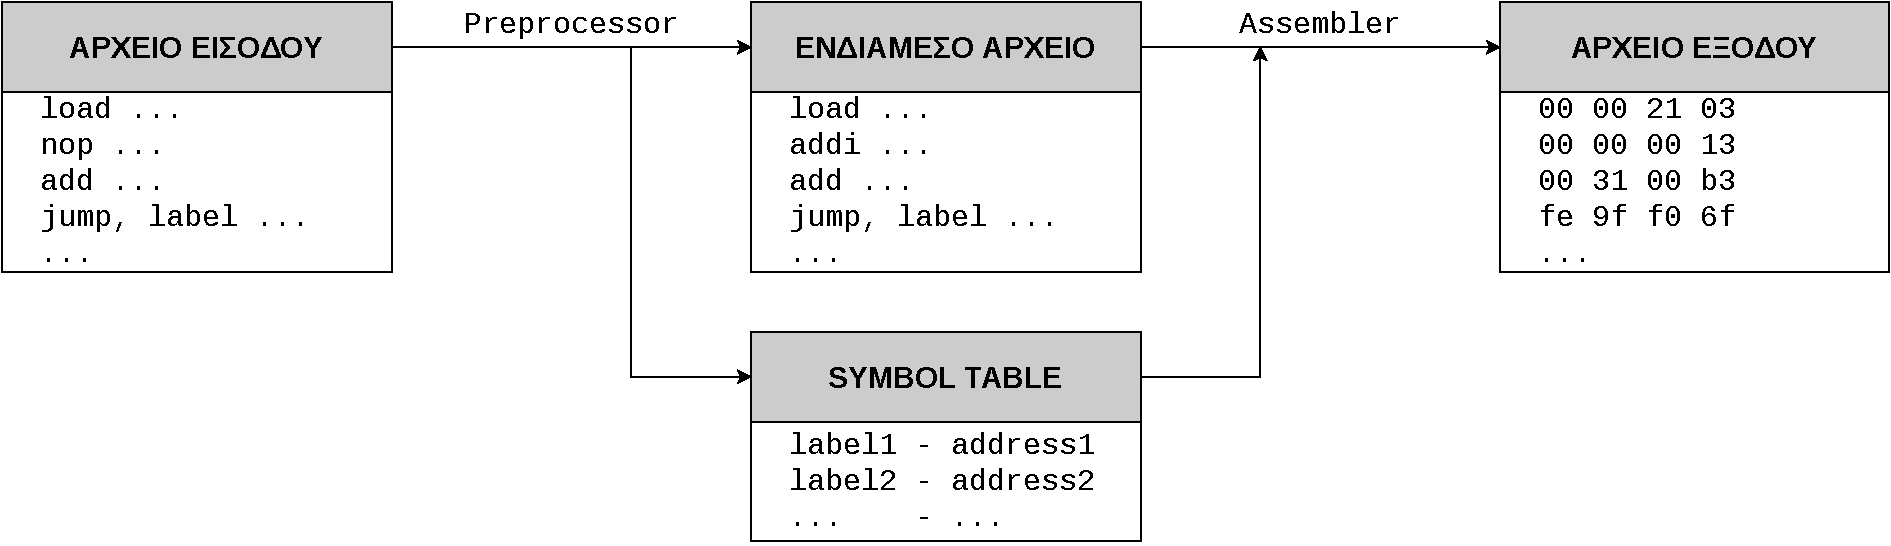
\includegraphics[width=\textwidth]{diagrams/assembler/assembler-preprocessor.pdf}}
    \caption[Assembly σε Εκτελέσιμο]{Διαδικασία μετατροπής αρχείου Assembly σε εκτελέσιμο αρχείο - αρχείο με την δυαδική κωδικοποίηση των εντολών.}
\end{figure}

\newpage
\subsection{Μορφές Εντολών Γλώσσας Μηχανής}
Στον Preprocessor ορίζονται οι μορφές των εντολών που μπορεί να συναντηθούν στο αρχείο εισόδου.
Πιο συγκεκριμένα:
\begin{itemize}
\item Instruction Register, Immediate(Register)
\item Instruction Register, Register, Register
\item Instruction Register, Register, Immediate
\item Instruction Register, Register, Label
\item Instruction Register, Immediate
\item Instruction Register, Label
\end{itemize}
Για παράδειγμα, αντίστοιχα για κάθε μορφή εντολής:
\begin{itemize}
\item sw s0, 0(s1) 
\item add s0, ra, sp
\item add s1, sp, 1
\item beq s0, zero, overflow\_handler
\item lui t1, 0xff
\item jal ra, overflow\_handler
\end{itemize}
Στον Preprocessor επίσης ορίζεται η μορφή των δηλώσεων Label ως εξής:
\begin{itemize}
\item Label:
\end{itemize}
Για παράδειγμα:
\begin{itemize}
\item overflow\_handler:
\end{itemize}

\newpage
\subsubsection{Ονοματολογία Καταχωρητών}
Οι προδιαγραφές ορίζουν συγκεκριμένα ονόματα για κάθε καταχωρητή, καθώς και προτεινόμενες χρήσεις για τον καθένα από αυτούς\footnotemark.
Ο Assembler παρέχει υποστήριξη για την χρήση οποιουδήποτε από τα παρακάτω ονόματα για αναφορά σε κάποιον συγκεκριμένο καταχωρητή.
\footnotetext{Από τις επίσημες προδιαγραφές προτείνονται συγκεκριμένες χρήσεις για κάθε καταχωρητή, για σκοπούς μεταφραστών και compiler υψηλότερου επιπέδου γλωσσών προγραμματισμού.
Η στανταρισμένη χρήση καταχωρητών θα μπορούσε να αξιοποιηθεί από πολυπλοκότερα μοντέλα.
Στην παρούσα διπλωματική εργασία δεν ασχολούμαστε με την μετάφραση γλωσσών υψηλότερου επιπέδου.}
\begin{table}[H]
\centering
\begin{tabular}{|c|c|}
\hline
\cellcolor{lgray} \textbf{Καταχωρητής} & \cellcolor{lgray} \textbf{Ονομασίες} \\\hline
x0     & zero    \\\hline
x1     & ra      \\\hline
x2     & sp      \\\hline
x3     & gp      \\\hline
x4     & tp      \\\hline
x5     & t0      \\\hline
x6-7   & t1-2    \\\hline
x8     & s0 / fp \\\hline
x9     & s1      \\\hline
x10-11 & a0-1    \\\hline
x12-17 & a2-7    \\\hline
x18-27 & s2-11   \\\hline
x28-31 & t3-6    \\\hline
\end{tabular}
\caption[Ονομασίες Καταχωρητών]{\label{tab:widgets}Ονομασίες καταχωρητών (Από \cite{spec}).}
\end{table}
Ο καταχωρητής x0 / zero είναι ορισμένος από την αρχιτεκτονική RISC-V να επιστρέφει σταθερά την τιμή 0 στην ανάγνωσή του, και το περιεχόμενό του να παραμένει αμετάβλητο στις εγγραφές.
Συνεπώς, οι εντολές που χρησιμοποιούν αυτόν τον καταχωρητή για αποθήκευση του αποτελέσματός τους δεν αλλάζουν την κατάσταση του επεξεργαστή.
Τέτοιου τύπου εντολές ορίζονται από την αρχιτεκτονική RISC-V ως προαιρετικές εντολές HINT για την μέτρηση της απόδοσης του επεξεργαστή, αφού δεν επιφέρουν αλλαγές στην κατάστασή του.
Θεωρούμε πως η κατάσταση του επεξεργαστή ορίζεται από τα περιεχόμενα των μνημών δεδομένων και τα περιεχόμενα των καταχωρητών.
Αφού οι εντολές με καταχωρητή αποτελέσματος x0 δεν μεταβάλλουν την τιμή σε κάποιον καταχωρητή ή μνήμη, δεν αλλάζουν και την κατάσταση του επεξεργαστή \cite{spec}.

\newpage
\subsection{Ψευδοεντολές}
O Preprocessor μπορεί να παραμετροποιηθεί για την υποστήριξη ψευδοεντολών.
Αναλαμβάνει την μετατροπή της ψευδοεντολής σε μια εντολή - ή μια ακολουθία εντολών - κατάλληλη για περαιτέρω μετατροπή της στην δυαδική κωδικοποίησή της από τον Assembler.
Μία τέτοια ψευδοεντολή που έχει υλοποιηθεί είναι η εντολή "nop" (No Operation), που είναι ορισμένη ως την εντολή "addi x0, x0, 0" (add immediate - x0 \textleftarrow\space x0 + 0) με βάση τις προδιαγραφές της αρχιτεκτονικής RISC-V.
Ο Preprocessor, εντοπίζοντας την ψευδοεντολή "nop", καταγράφει στο ενδιάμεσο αρχείο την αποκωδικοποίηση της ψευδοεντολής σε μια απλή μορφή εντολής Assembly, δηλαδή "addi x0, x0, 0", που μπορεί να επεξεργαστεί ο Assembler. 
Για ακολουθίες εντολών που παράγονται από μία μόνο ψευδοεντολή είναι απαραίτητο να εφαρμοστεί διόρθωση στην τιμή του μετρητή θέσεων μνήμης, καθώς ο Preprocessor αυξάνει τον μετρητή κατά 4 για κάθε εντολή ή ψευδοεντολή που υπάρχει στο αρχείο εισόδου. Είναι σημαντικό να αναφερθεί πως τα Labels δεν αποτελούν εντολές προς εκτέλεση, οπότε δεν μεταβάλλουν τον μετρητή θέσεων μνήμης.
\begin{figure}[H]
    \centering
    \makebox[\textwidth][c]{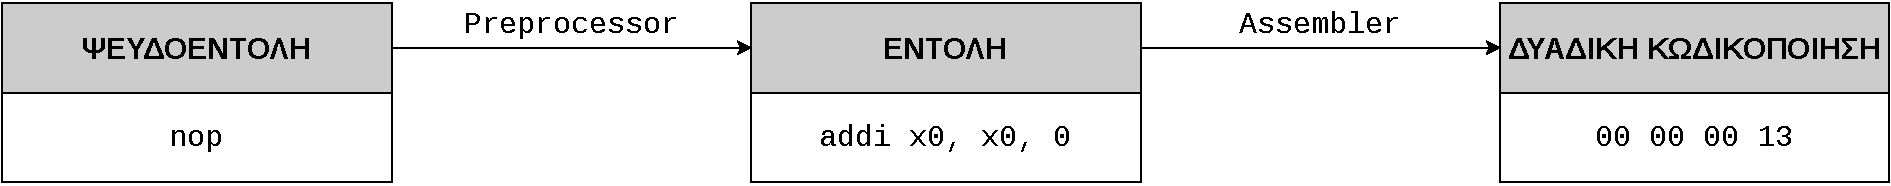
\includegraphics[width=\textwidth]{diagrams/assembler/pseudoinstruction.pdf}}
    \caption[Αποκωδικοποίηση Ψευδοεντολής]{Διαδικασία αποκωδικοποίησης ψευδοεντολής και μετατροπή της σε δυαδική κωδικοποίηση.}
\end{figure}

\subsection{Ο Ρόλος του Assembler στις Εντολές Διακλάδωσης - Υλοποίηση των Label}
Στις προδιαγραφές των RISC-V επεξεργαστών (πέραν της επέκτασης C - Compressed, στην οποία κάθε εντολή μπορεί να έχει διαφορετικό μήκος) κάθε εντολή έχει μήκος 32 bit (4 byte), ανεξάρτητα από το μέγεθος του εντέλου του επεξεργαστή.
Η διευθυνσιοδότηση της μνήμης εντολών γίνεται ανά byte, συνεπώς κάθε μία εντολή καταλαμβάνει 4 θέσεις μνήμης.
Ο Preprocessor αναγιγνώσκει το περιεχόμενο του αρχείου εισόδου χωρίζοντάς το σε "λέξεις". 
Εφόσον ένα σύνολο λέξεων ακολουθεί την γραμματική και την δομή μίας από τις μορφές των εντολών, εγγράφεται η αντίστοιχη μερικώς επεξεργασμένη εντολή στο παραγόμενο από τον Preprocessor αρχείο από τον Assembler.
Ο Preprocessor χρησιμοποιεί έναν μετρητή θέσεων μνήμης για κάθε εντολή ο οποίος ξεκινάει από το 0 και για κάθε εντολή που επεξεργάζεται, αυξάνεται κατά 4.

Σε περίπτωση που βρεθεί ο ορισμός ενός Label, καταγράφεται το όνομά του και η θέση μνήμης του, δηλαδή η διεύθυνση μνήμης της εντολής στην οποία αναφέρεται.
Ο Preprocessor δηλαδή, κατασκευάζει μια απλουστευμένη μορφή ενός symbol table, με τα ονόματα και τις διευθύνσεις μνήμης των ονοματισμένων σημείων των υπο-ρουτινών στο αρχείο εισόδου. 
Είναι απαραίτητο το ίδιο το Label να μη προσμετρηθεί στην καταμέτρηση των θέσεων μνήμης καθώς δεν αποτελεί εντολή προς τον επεξεργαστή και δεν καταλαμβάνει χώρο στην μνήμη εντολών.
Τα labels αξιοποιούνται για να διευκολυνθεί ο προγραμματισμός του επεξεργαστή. 
Χρησιμοποιούνται για τον "ονοματισμό" θέσεων του κώδικα και αυτοματοποιούν τον υπολογισμό των θέσεων μνήμης για τις εντολές διακλάδωσης.
Αφού ολοκληρωθεί η προ-επεξεργασία του αρχικού αρχείου εισόδου, έχει δημιουργηθεί το ενδιάμεσο αρχείο που θα χρησιμοποιηθεί ως είσοδος του Assembler.

Πέραν του ενδιάμεσου αρχείου, ο Assembler αξιοποιεί το symbol table που δημιουργεί ο Preprocessor για την αποκωδικοποίηση των εντολών που χρημιοποιούν Label.
Οι εντολές διακλάδωσης της αρχιτεκτονικής RISC-V χρησιμοποιούν σχετική διευθυνσιοδότηση για να δίνουν την δυνατότητα στα προγράμματα να βρίσκονται σε οποιαδήποτε θέση μνήμης.
Η διέυθυνση μνήμης στην οποία πρόκεται να γίνει η διακλάδωση υπολογίζεται με βάση την τρέχουσα διεύθυνση μνήμης που βρίσκεται στον μετρητή προγράμματος.
Ο Assembler, έχοντας την πληροφορία που παρέχεται από το symbol table, παράγει το σωστό Offset το οποίο θα προστεθεί στην διεύθυνση μνήμης του μετρητή προγράμματος, έτσι ώστε να αποκτήσει την διεύθυνση της επόμενης εντολής που υποδεικνύεται από την εντολή διακλάδωσης.
Το offset πρόκειται για την διαφορά της διεύθυνσης μνήμης της τρέχουσας εντολής από την διεύθυνση μνήμης της επιθυμητής εντολής της οποίας πρόκειται να εκτελεστεί εφόσον η συνθήκη διακλάδωσης αληθεύει.
Με την τεχνική του σχετικού υπολογισμού της θέσης μνήμης διακλάδωσης εξασφαλίζεται με απλό τρόπο πως το πρόγραμμα που αποκωδικοποιεί ο Preprocessor και ο Assembler θα εκτελεστεί σωστά, ανεξαρτήτως της θέσης που βρίσκεται στην μνήμη προγράμματος.
Αυτό συμβαίνει λόγω του γεγονότος πως οι διευθύνσεις των διακλαδώσεων υπολογίζονται σε σχέση με την διεύθυνση της τρέχουσας εντολής.
\begin{table}[H]
\centering
\begin{tabular}{|l|c|}
\hline
\cellcolor{lgray} \textbf{Όνομα Label} & \cellcolor{lgray} \textbf{Θέση μνήμης} \\\hline
\_\_start         & 0x8000 \\\hline
overflow\_handler & 0x8040 \\\hline
stack\_pop        & 0x8100 \\\hline
...               & ...    \\\hline
\end{tabular}
\caption[Symbol Table]{\label{tab:widgets}Ένα απλό παράδειγμα του symbol table.}
\end{table}

\newpage
\subsection{Παραγωγή Διανυσμάτων Εντολών}
Τα διανύσματα εντολών που παράγονται από τον Assembler αξιοποιούν τον τύπο δεδομένων \textbf{unsigned int} μήκους \textbf{32 bit}, και δημιουργούνται με ολισθήσεις και προσθέσεις.
Η αποθήκευση των παραγόμενων διανυσμάτων εντολών στο αρχείο εξόδου μπορεί να γίνει είτε σε δυαδική μορφή για την παραγωγή δυαδικών εκτελέσιμων αρχείων με μια μικρή παραμετροποίηση του Assembler, είτε σε μορφή ASCII που χρησιμοποιείται στο τρέχον μοντέλο, για την φόρτωσή τους στην μνήμη εντολών.

\begin{table}[H]
\makebox[\textwidth][c]{
\begin{tabular}{p{0.2\textwidth} p{0.15\textwidth} p{0.15\textwidth} p{0.1\textwidth} p{0.15\textwidth} p{0.20\textwidth} p{0.1\textwidth}}
\instbitrange{31}{25} &
\instbitrange{24}{20} &
\instbitrange{19}{15} &
\instbitrange{14}{12} &
\instbitrange{11}{7}  &
\instbitrange{6}{0}   &  \\\cline{1-6}
\multicolumn{1}{|c|}{funct7} &
\multicolumn{1}{c|}{rs2} &
\multicolumn{1}{c|}{rs1} &
\multicolumn{1}{c|}{funct3} &
\multicolumn{1}{c|}{rd} &
\multicolumn{1}{c|}{opcode} &
\multicolumn{1}{l}{R - type} \\\cline{1-6}
\multicolumn{1}{|c|}{0000000} &
\multicolumn{1}{c|}{00010} &
\multicolumn{1}{c|}{00001} &
\multicolumn{1}{c|}{000} &
\multicolumn{1}{c|}{00011} &
\multicolumn{1}{c|}{0110011} &
\multicolumn{1}{l}{add x3, x1, x2} \\\cline{1-6} \\
\hline\\
\multicolumn{7}{l}{
    Αρχικά, δεν έχει οριστεί κάποια τιμή στο διάνυσμα της εντολής.
} \\\cline {1-6}
\multicolumn{1}{|c|}{xxxxxxx} &
\multicolumn{1}{c|}{xxxxx} &
\multicolumn{1}{c|}{xxxxx} &
\multicolumn{1}{c|}{xxx} &
\multicolumn{1}{c|}{xxxxx} &
\multicolumn{1}{c|}{xxxxxxx} &
\multicolumn{1}{l}{Αρχικά}\\\cline{1-6} \\
\hline\\
\multicolumn{7}{l}{
    Θέτουμε την τιμή του opcode στο διάνυσμα της εντολής.
} \\\cline {1-6}
\multicolumn{1}{|c|}{xxxxxxx} &
\multicolumn{1}{c|}{xxxxx} &
\multicolumn{1}{c|}{xxxxx} &
\multicolumn{1}{c|}{xxx} &
\multicolumn{1}{c|}{xxxxx} &
\multicolumn{1}{c|}{\textbf{0110011}} &
\multicolumn{1}{l}{1 - opcode}\\\cline{1-6} \\
\hline\\
\multicolumn{7}{p{1.1\textwidth}}{
    Προσθέτουμε την τιμή του επόμενου πεδίου (rd = 00011\textsubscript{b}) \textbf{αριστερά ολισθημένη κατά το μέγεθος του προηγούμενου πεδίου} στο αποτέλεσμα του βήματος 1. 
    Στην συγκεκριμένη περίπτωση το πεδίο opcode έχει μέγεθος 7 bit συνεπώς θα γίνει ολίσθηση στην τιμή rd κατά 7 ψηφία αριστερά.
    Αυτή η διαδικασία ολίσθησης και πρόσθεσης μεταβάλλει μόνο το επόμενο πεδίο του διανύσματος διατηρώντας τα δεξιότερα ψηφία αμετάβλητα.
} \\\cline {1-6}
\multicolumn{1}{|c|}{xxxxxxx} &
\multicolumn{1}{c|}{xxxxx} &
\multicolumn{1}{c|}{xxxxx} &
\multicolumn{1}{c|}{xxx} &
\multicolumn{1}{c|}{\textbf{00011}} &
\multicolumn{1}{c|}{0110011} &
\multicolumn{1}{l}{2 - rd} \\\cline{1-6} \\
\hline\\
\multicolumn{7}{p{1.1\textwidth}}{
    Επαναλαμβάνουμε την παραπάνω διαδικασία ολίσθησης και πρόσθεσης για τα υπόλοιπα πεδία της εντολής.
} \\\cline {1-6}
\multicolumn{1}{|c|}{xxxxxxx} &
\multicolumn{1}{c|}{xxxxx} &
\multicolumn{1}{c|}{xxxxx} &
\multicolumn{1}{c|}{\textbf{000}} &
\multicolumn{1}{c|}{00011} &
\multicolumn{1}{c|}{0110011} &
\multicolumn{1}{l}{3 - funct3} \\\cline{1-6}
\multicolumn{1}{|c|}{xxxxxxx} &
\multicolumn{1}{c|}{xxxxx} &
\multicolumn{1}{c|}{\textbf{00001}} &
\multicolumn{1}{c|}{000} &
\multicolumn{1}{c|}{00011} &
\multicolumn{1}{c|}{0110011} &
\multicolumn{1}{l}{4 - rs1} \\\cline{1-6}
\multicolumn{1}{|c|}{xxxxxxx} &
\multicolumn{1}{c|}{\textbf{00010}} &
\multicolumn{1}{c|}{00001} &
\multicolumn{1}{c|}{000} &
\multicolumn{1}{c|}{00011} &
\multicolumn{1}{c|}{0110011} &
\multicolumn{1}{l}{5 - rs2} \\\cline{1-6}
\multicolumn{1}{|c|}{\textbf{0000000}} &
\multicolumn{1}{c|}{00010} &
\multicolumn{1}{c|}{00001} &
\multicolumn{1}{c|}{000} &
\multicolumn{1}{c|}{00011} &
\multicolumn{1}{c|}{0110011} &
\multicolumn{1}{l}{6 - funct7} \\\cline{1-6}
\end{tabular}
}
\caption[Παράδειγμα - Παραγωγή Διανύσματος add]{\label{tab:widgets}Διαδικασία αποκωδικοποίησης και παραγωγής του διανύσματος της εντολής add x3, x1, x2}
\end{table}

\subsection{Περαιτέρω Παραμετροποίηση}
Αξιοποιώντας την υπάρχουσα τεχνική ολίσθησης - πρόσθεσης δίνεται η δυνατότητα να προστεθεί στον Assembler υποστήριξη για οποιαδήποτε μορφή εντολής στο επίπεδο της δυαδικής κωδικοποίησης.
Με τροποποίηση του Preprocessor μπορούν επίσης να υλοποιηθούν ευκολότερα μνημονικά και μορφές εντολών της γλώσσας Assembly για την διευκόλυνση του προγραμματισμού του επεξεργαστή. 

Ένα παράδειγμα είναι η χρήση απλών μαθηματικών τύπων για αντικατάσταση των μνημονικών των εντολών αριθμητικών πράξεων.
Μια εντολή με πιο ασυνήθιστη γραμματική μορφή "x3 = x1 + x2" θα μπορούσε να μετατρέπεται από τον Preprocessor στην ήδη υποστηριζόμενη από τον Assembler μορφή "add x3, x1, x2".

\section{ΕΠΕΞΕΡΓΑΣΤΗΣ - ΣΧΕΔΙΑΣΤΙΚΕΣ ΑΠΟΦΑΣΕΙΣ}
Σε αυτό το κεφάλαιο παρουσιάζεται η συλλογιστική πορεία που ακολουθήθηκε στην σχεδίαση του μοντέλου του επεξεργαστή.
Οι αποφάσεις αιτιολογούνται με βάση την ανάλυση των εντολών της βασικής αρχιτεκτονικής συνόλου εντολών RV32I, καθώς και με την ακολούθηση ορισμένων σχεδιαστικών τάσεων και τεχνικών από άλλες υλοποιήσεις RISC επεξεργαστών και επεξεργαστών γενικότερα.

\subsection{Η τεχνική της διασωλήνωσης}
Οι περισσότεροι RISC επεξεργαστές αποφεύγουν την χρήση μικροκώδικα και αξιοποιούν την τεχνική της διασωλήνωσης στην μικροαρχιτεκτονική τους.
Η τεχνική της διασωλήνωσης χωρίζει τις επιμέρους υπολειτουργίες μιας εντολής σε στάδια, τα οποία εκτελούνται το ένα μετά το άλλο.
Η εκτέλεση ενός σταδίου είναι ανεξάρτητη από τα άλλα, και έτσι επιτυγχάνεται ένας βαθμός παραλληλοποίησης σε επίπεδο εντολής \cite{patterson}. \newline

Τα πέντε στάδια της κλασσικής διασωλήνωσης RISC είναι τα εξής \cite{nikolos}:
\begin{description}
    \item[IF - Instruction Fetch] Ανάκτηση εντολής \newline
    Σε αυτο το στάδιο γίνεται ανάγνωση της εντολής προς εκτέλεση.
    Ο μετρητής προγράμματος επίσης αυξάνεται ανάλογα, έτσι ώστε να διευθυνσιοδοτεί την επόμενη εντολή προς εκτέλεση και να αναγνωστεί στον επόμενο κύκλο.
    \item[ID - Instruction Decode] Αποκωδικοποίηση εντολής \newline
    Μετά την ανάγνωση της εντολής, γίνεται ανάγνωση του περιεχομένου των καταχωρητών τους οποίους ορίζει η εντολή.
    Τα δεδομένα ανάγνωσης θα προχωρήσουν προς το επόμενο στάδιο για περαιτέρω επεξεργασία.
    \item[EX - Execute] Εκτέλεση \newline
    Στο στάδιο της εκτέλεσης εφαρμόζεται η πράξη που έχει οριστεί από την εντολή στα δεδομένα από τους καταχωρητές που έχουν αναγνωστεί.
    Το αποτέλεσμα μπορεί να είναι ένα αριθμητικό δεδομένο ή ένας υπολογισμός διεύθυνσης για την προσπέλαση της μνήμης δεδομένων.
    Στην περίπτωση που εκτελείται πράξη με αριθμητικό αποτέλεσμα, θα χρειαστεί να αποθηκευτεί σε έναν καταχωρητή σε επόμενο στάδιο της διασωλήνωσης (στάδιο WB).
    Στην περίπτωση υπολογισμού διεύθυνσης, το αποτέλεσμα του υπολογισμού προχωράει στο στάδιο MEM.
    \item[MEM - Memory Access] Προσπέλαση Μνήμης \newline
    Σε αυτό το στάδιο γίνεται η προσπέλαση της μνήμης δεδομένων, αφότου έχει υπολογιστεί η διεύθυνση προσπέλασης στο στάδιο EX.
    Σε περίπτωση που εκτελείται εντολή ανάγνωσης, το δεδομένο αποθηκεύεται σε έναν καταχωρητή αποτελέσματος για να εγγραφεί στο αρχείο καταχωρητών κατά το επόμενο στάδιο εκτέλεσης.
    Σε περίπτωση εντολής εγγραφής στην μνήμη, το δεδομένο προς εγγραφή είναι προετοιμασμένο από τους προηγούμενους κύκλους.
    \item[WB - Write Back\footnotemark] Επανεγγραφή \newline
    Στο τελευταίο στάδιο της διασωλήνωσης γίνεται η εγγραφή του αριθμητικού αποτελέσματος της πράξης που ορίζει η εντολή (από το στάδιο ΕΧ) ή το δεδομένο από την ανάγνωση της μνήμης (στο στάδιο MEM) στους καταχωρητές.
\end{description}
\footnotetext{Στην συγκεκριμένη υλοποίηση, το στάδιο MEM συγχωνεύεται με το στάδιο WB. Αξιοποιώντας την προκαθορισμένη συμπεριφορά του εξομοιωτή Icarus Verilog παρατηρήθηκε πως η ανάγνωση της μνήμης και η εγγραφή του αποτελέσματος στον καταχωρητή μπορούν να εκτελεστούν ταυτόχρονα.}

\newpage

Καθώς οι λειτουργίες της διασωλήνωσης είναι μερικώς επικαλυπτόμενες, ο σχεδιασμός του μοντέλου του επεξεργαστή οφείλει να αντιμετωπίζει τυχόντα προβλήματα που δημιουργούνται από αυτή την επικάλυψη λειτουργιών.
Ειδικότερα στην περίπτωση που θέλουμε ο επεξεργαστής να είναι απόλυτα συμβατός με την αρχιτεκτονική RV32I, η οποία δεν ορίζει καμία ακολουθία εντολών εκτός προδιαγραφών, τα προβλήματα που δημιουργούνται από την διασωλήνωση θα πρέπει να αντιμετωπίζονται σε κάθε περίπτωση στο επίπεδο του υλικού.



\subsection{Επιμέρους Λειτουργικές Μονάδες}
Θεωρείται πως όλες οι μονάδες υλοποιούνται ως ακολουθιακά κυκλώματα και λειτουργούν με σήμα ρολογιού, εκτός αν αναφέρεται διαφορετικά.
Για κάθε λειτουργική μονάδα έχουμε θεωρήσει πως χρειάζεται έναν κύκλο ρολογιού για να εκτελέσει την λειτουργία της, και πως είναι θετικά ακμοπυροδότητη.
Η θύρα εισόδου του σήματος ρολογιού παραλείπεται από τις περιγραφές.

\subsubsection{Μνήμη}
Αρχικά, χρειαζόμαστε μια μονάδα για την ανάγνωση των εντολών προς εκτέλεση.
Με αυτήν την μονάδα, ο επεξεργαστής αλληλεπιδρά μόνο μέσω του μετρητή προγράμματος ο οποίος την διευθυνσιοδοτεί έτσι ώστε να αναγνωστεί η εντολή προς εκτέλεση.
Χρειαζόμαστε επίσης μια μονάδα μνήμης για την ανάγνωση και την εγγραφή δεδομένων κατά την εκτέλεση του προγράμματος.

Παρατηρώντας το σύνολο εντολών που αφορούν την μνήμη (κατηγορία εντολών Load - Store), συμπεραίνουμε πως δεν υπάρχει καμία εντολή η οποία χρειάζεται να κάνει εγγραφή και ανάγνωση της μνήμης δεδομένων ταυτόχρονα.
Συνεπώς, μπορούμε να χρησιμοποιήσουμε μια θύρα δεδομένων, η οποία εκτελεί μία λειτουργία ανάγνωσης ή εγγραφής σε κάθε κύκλο.
Για τον καθορισμό της λειτουργίας της μνήμης χρησιμοποιείται ένα σήμα εγγραφής ή ανάγνωσης, ανάλογα με τις ανάγκες της εντολής.
Η προσπέλαση της μνήμης προϋποθέτει επίσης τον ορισμό της διεύθυνσης προς προσπέλαση, άρα και μια θύρα διεύθυνσης.

Υπάρχουν πολλές εντολές εγγραφής (sb, sh, sw), με ειδοποιό διαφορά το μέγεθος του δεδομένου προς εγγραφή.
Η διαφορά αυτή είναι κβαντισμένη ανά byte όσο αναφορά το μέγεθος της εγγραφής και κωδικοποιείται στο πεδίο funct3 του διανύσματος της εντολής.
Αυτό οδηγεί αρχικά στην απόφαση διευθυνσιοδότησης της μνήμης ανά byte, και επίσης στον ορισμό μιας θύρας που καθορίζει το μέγεθος της εγγραφής.

Με τον ίδιο τρόπο ορίζονται από τις προδιαγραφές και οι εντολές ανάγνωσης της μνήμης (lb, lh, lw), με την προσθήκη όμως μιας απλής επέκτασης προσήμου πριν την εγγραφή του αναγιγνωσμένου δεδομένου στον ορισμένο καταχωρητή. Υπάρχουν και οι αντίστοιχες εντολές οι οποίες δεν κάνουν επέκταση προσήμου (lbu, lhu).
Αφού και αυτές οι λειτουργίες κωδικοποιούνται στο πεδίο funct3 της εντολής, η μνήμη αναλαμβάνει επίσης και την επέκταση προσήμου στις λειτουργίες ανάγνωσης που επιβάλλεται, με βάση την τιμή αυτής της θύρας. 

Ο τρέχων σχεδιασμός της μνήμης δεδομένων υπερκαλύπτει τις ανάγκες της μνήμης εντολών, άρα χρησιμοποιούμε την ίδια λειτουργική μονάδα και για τις δύο μνήμες.
Η μνήμη εντολών είναι ορισμένη να εκτελεί μόνο λειτουργίες ανάγνωσης μεγέθους 32 bit\footnotemark, δηλαδή την εντολή lw, μέσω κατάλληλα ορισμένων τιμών στις θύρες της.
\footnotetext{Το σταθερό μέγεθος των 32 bit είναι ορισμένο από τις προδιαγραφές ως το μέγεθος των διανυσμάτων των εντολών της αρχιτεκτονικής RV32I.}
\newline

\newpage
Καταλήγουμε στον παρακάτω σχεδιασμό:
\begin{figure}[H]
    \centering
    \makebox[\textwidth][c]{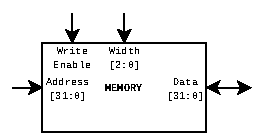
\includegraphics[scale=2]{diagrams/cpu/mem.pdf}}
    \caption[Μονάδα Μνήμης]{Η μονάδα μνήμης}
\end{figure}
Ο επεξεργαστής διαθέτει δύο μνήμες, Μνήμη Εντολών και Μνήμη Δεδομένων, βασιζόμενες στην ίδια λειτουργική μονάδα.
Η μονάδα μνήμης διευθυνσιοδοτείται ανά byte και μπορεί να αποθηκεύσει και να αναγνώσει λέξεις μεταβλητού μεγέθους 1, 2, 4 και 8 byte σε έναν κύκλο. 
Η μονάδα μπορεί να εφαρμόσει επέκταση προσήμου στην θύρα εξόδου των δεδομένων, εφόσον το μέγεθος της ανάγνωσης δεν καλύπτει το μέγιστο μέγεθος των 4 ή 8 byte (Ίσο με το μέγεθος του εντέλου του επεξεργαστή).
\vspace{1em}
\newline
\textit{Διαθέτει τις εξής θύρες εισόδου:}
\begin{description}
 \item[Address] Μεταβλητό μέγεθος, ανάλογο με το μέγεθος της μνήμης. \newline
 Χρησιμοποιείται για την επιλογή της διεύθυνσης της λέξης.
 \item[Width] Σήμα μεγέθους λειτουργίας μεγέθους 3 bit. \newline
 Χρησιμοποιείται για την επιλογή του μεγέθους της ανάγνωσης ή της εγγραφής. 
 Η λειτουργία (εγγραφή ή ανάγνωση) γίνεται στην δοθείσα διεύθυνση [Address] και στις αμέσως επόμενες ανάλογα με την τιμή του μεγέθους που δίνεται.
 Εφαρμόζεται επίσης επέκταση προσήμου ανάλογα με την τιμή του [Width].
 \begin{itemize}
    \item Εάν το πιο σημαντικό bit έχει την τιμή 0, εφαρμόζεται επέκταση προσήμου στην λέξη προς ανάγνωση. 
    \item Διαφορετικά, οι κενές θέσεις τιμοδοτούνται με 0.
 \end{itemize}
 Δεν εφαρμόζεται κάποια επέκταση προσήμου στις λειτουργίες εγγραφής.
 \item[Write Enable] Σήμα λειτουργίας ανάγνωσης/εγγραφής ενός bit. \newline
 Χρησιμοποιείται για την επιλογή της λειτουργίας της μνήμης. 
 Οι ενέργειες αφορούν το περιεχόμενο στην διεύθυνση μνήμης που δίνεται στην θύρα [Address]. 
 \begin{itemize}
     \item Εάν το σήμα έχει τιμή 0, γίνεται ανάγνωση του περιεχομένου της θέσης μνήμης [Address], καθώς και στις αμέσως επόμενες ανάλογα με την τιμή της θύρας [Width].
     \item Εάν το σήμα έχει τιμή 1, γίνεται εγγραφή του περιεχομένου της θύρας [Data] στην θέση μνήμης [Address], καθώς και στις αμέσως επόμενες ανάλογα με την τιμή της θύρας [Width].
 \end{itemize}
\end{description}
\newpage
\textit{Διαθέτει την εξής θύρα εισόδου/εξόδου:}
\begin{description}
 \item[Data] Θύρα εισόδου/εξόδου δεδομένου μεταβλητού μεγέθους. \newline
 Η λειτουργικότητα της θύρας καθορίζεται από το σήμα [Write Enable]. 
 Το μέγεθος της λέξης ανάγνωσης ή της λέξης προς εγγραφή καθορίζεται από την τιμή στην θύρα [Width]. 
 \begin{itemize}
 \item Εάν το σήμα [Write Enable] έχει τιμή 0, λειτουργεί ως θύρα εξόδου και παίρνει την τιμή του περιεχομένου της θέσης μνήμης [Address].
 \item Εάν το σήμα [Write Enable] έχει τιμή 1, λειτουργεί ως θύρα εισόδου και γίνεται εγγραφή του περιεχομένου της στην θέση μνήμης [Address].
 \end{itemize}
 Σημειώνεται πως δεν υπάρχει δυνατότητα ταυτόχρονης ανάγνωσης και εγγραφής.
\end{description}

\subsubsection{Αριθμητική - Λογική Μονάδα}
Σε κάθε περίπτωση των εντολών εκτέλεσης αριθμητικών - λογικών πράξεων, υπάρχουν μόνο δύο δεδομένα και μια εκτέλεση πράξης.
Αυτό ορίζει δύο θύρες για τα δεδομένα που θα εκτελεστεί η πράξη και μια θύρα αποτελέσματος της πράξης.
Η εκτέλεση της πράξης ορίζεται από το πεδίο funct3 και προαιρετικά το πεδίο funct7 όπου χρειάζεται, άρα η μονάδα θα χρειαστεί επίσης μια θύρα για τον ορισμό της πράξης προς εκτέλεση.

Η διαφορά των πράξεων Register - Register και Register - Immediate καθορίζεται από το πεδίο opcode, ωστόσο δεν επηρεάζει την λειτουργία της Αριθμητικής - Λογικής μονάδας καθώς εξακολουθεί να εφαρμόζει μια πράξη σε 2 δεδομένα. \newline

Υπάρχουν περιπτώσεις όπου απαιτείται υπολογισμός πράξης σε εντολές που δεν ανήκουν στην κατηγορία αριθμητικών - λογικών πράξεων:
\begin{itemize}
    \item Σε κάθε περίπτωση διευθυνσιοδότησης της μνήμης, δηλαδή στις εντολές \textbf{Load, Store}, η αριθμητική - λογική μονάδα αξιοποιείται για τον υπολογισμό της διεύθυνσης κάνοντας την πρόσθεση του άμεσου δεδομένου με το δεδομένο που αναγιγνώσθηκε από τον καταχωρητή που ορίζει η εντολή.
    \item Στην εντολή \textbf{jal} απαιτείται επίσης μια πρόσθεση του άμεσου δεδομένου label που βρίσκεται κωδικοποιημένο στο διάνυσμα της εντολής με το δεδομένου του καταχωρητή που ορίζεται από την εντολή.
    \item Στην εντολή \textbf{auipc} απαιτείται η πρόσθεση του περιεχομένου του μετρητή προγράμματος στο δεδομένο ενός καταχωρητή που ορίζει η εντολή.
\end{itemize}
Σε κάθε περίπτωση δηλαδή που δεν εφαρμόζεται μια ορισμένη από την εντολή αριθμητική - λογική πράξη, μπορούμε να αποφασίσουμε πως η αριθμητική - λογική μονάδα θα εκτελεί την πράξη της πρόσθεσης στα δύο δεδομένα που της δίνονται. \newline
\newpage
Συνεπώς, η σχεδίαση της αριθμητικής - λογικής μονάδας είναι:
\begin{figure}[H]
    \centering
    \makebox[\textwidth][c]{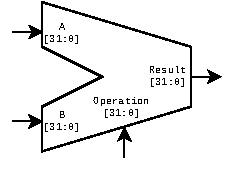
\includegraphics[scale=2]{diagrams/cpu/alu.pdf}}
    \caption[Αριθμητική - Λογική Μονάδα]{Η αριθμητική - λογική μονάδα}
\end{figure}
Η μονάδα χρησιμοποιείται για αριθμητικές και λογικές πράξεις μεταξύ δύο έντελων. 
Υποστηρίζει αριθμητικές πράξεις ακεραίων (integer operations), λογικές πράξεις ανά bit (bitwise logic operations) συμπεριλαμβανομένων αριθμητικών και λογικών ολισθήσεων (arithmetic - logical shift).
\vspace{1em}
\newline
\textit{Διαθέτει τις εξής θύρες εισόδου:}
\begin{description}
 \item[Θύρα A και Θύρα B] Θύρα εισόδου εντέλου σταθερού μεγέθους, ανάλογο με το μέγεθος του εντέλου του επεξεργαστή (32 ή 64 bit). \newline
 Σε αυτές τις θύρες δίνονται οι τιμές των εντέλων για την εκτέλεση της πράξης.
 \item[Operation] Θύρα εισόδου πράξης μεγέθους 32 bit. \newline
 Ανάλογα με την τιμή της θύρας, εφαρμόζεται μια συγκεκριμένη πράξη μεταξύ των εντέλων Α και Β.
 Σε περίπτωση που δεν έχει οριστεί συγκεκριμένη πράξη, εκτελείται η πράξη της πρόσθεσης.
\end{description}
\textit{Διαθέτει την εξής θύρα εξόδου:}
\begin{description}
 \item[Result] Θύρα εξόδου αποτελέσματος σταθερού μεγέθους, ανάλογο με το μέγεθος του εντέλου του επεξεργαστή (32 ή 64 bit). \newline
Αυτή η θύρα τιμοδοτείται με το αποτέλεσμα της πράξης [Α] [Operation] [B], στον επόμενο κύκλο ρολογιού. 
\end{description}


\subsubsection{Αρχείο Καταχωρητών}
Σχεδόν σε όλες τις κωδικοποιήσεις εντολών υπάρχει το πεδίο rs1, το οποίο ορίζει έναν καταχωρητή προς ανάγνωση, και το πεδίο rd που ορίζει τον καταχωρητή προς εγγραφή του αποτελέσματος.
Σε αρκετές κωδικοποιήσεις επίσης υπάρχει το πεδίο rs2, το οποίο ορίζει έναν δεύτερο καταχωρητή προς ανάγνωση.
Με βάση τα παραπάνω, ορίζουμε στο αρχείο καταχωρητών 3 θύρες διευθύνσεων, 2 για ανάγνωση και 1 για εγγραφή.
Αντίστοιχα ορίζονται 2 θύρες δεδομένων ανάγνωσης των αντίστοιχων καταχωρητών και 1 θύρα δεδομένων εγγραφής σε καταχωρητή.
Τα μεγέθη των θυρών διευθύνσεων ορίζονται στα 5 bit, ίδιο μέγεθος με τα πεδία rs1, rs2, rd, αφού οι προδιαγραφές ορίζουν 32 καταχωρητές.
Ορίζουμε επίσης μια θύρα ενεργοποίησης εγγραφής, καθώς δεν απαιτείται εγγραφή του αποτελέσματος σε καταχωρητή σε κάθε εντολή.

Η διασωλήνωση επιβάλλει ταυτόχρονη εγγραφή και ανάγνωση του αρχείου καταχωρητών, για την αποφυγή δομικών κινδύνων.
Οι δομικοί κίνδυνοι προκύπτουν όταν μία μονάδα αξιοποιείται σε παραπάνω από ένα στάδιο της διασωλήνωσης \cite{nikolos}.
Στην συγκεκριμένη περίπτωση, τα στάδια όπου αξιοποιείται ταυτόχρονα κάποια μονάδα, είναι τα στάδια MEM/WB και ID.

Στην συγκεκριμένη υλοποίηση αξιοποιείται η προκαθορισμένη συμπεριφορά του εξομοιωτή Icarus Verilog για ταυτόχρονη ανάγνωση και εγγραφή στον ίδιο καταχωρητή, η οποία επιτρέπει την ταυτόχρονη ανάγνωση και εγγραφή στον ίδιο κύκλο, με προτεραιότητα στο δεδομένο προς εγγραφή.
Η συμπεριφορά αυτή λύνει το δομικό πρόβλημα που παρουσιάζεται, ενώ ταυτόχρονα προσομοιώνει πραγματικές υλοποιήσεις επεξεργαστών \cite{patterson}. \newline

Τα παραπάνω οδηγούν σε αυτήν την σχεδίαση αρχείου καταχωρητών:
\begin{figure}[H]
    \centering
    \makebox[\textwidth][c]{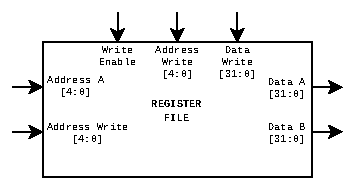
\includegraphics[scale=2]{diagrams/cpu/regfile.pdf}}
    \caption[Αρχείο Καταχωρητών]{Το αρχείο καταχωρητών}
\end{figure}
Το αρχείο καταχωρητών πρόκειται για ένα σύνολο 32 διευθυνσιοδοτημένων καταχωρητών, όπως είναι ορισμένο στις προδιαγραφές \cite{spec}.
Δίνεται η δυνατότητα ανάγνωσης του καταχωρητή στον ίδιο κύκλο εγγραφής του.
\vspace{1em}
\newline
\textit{Διαθέτει τις εξής θύρες εισόδου:}
\begin{description}
 \item[Address A και Address B] Θύρες εισόδου διευθύνσεων καταχωρητών προς ανάγνωση, μεγέθους 5 bit. 
 \item[Address Write] Θύρα εισόδου διεύθυνσης καταχωρητή προς εγγραφή, μεγέθους 5 bit. 
 \item[Data Write] Θύρα εισόδου δεδομένων προς εγγραφή στον καταχωρητή με διεύθυνση [Address]. \newline
 Το μέγεθος της θύρας καθορίζεται ανάλογα με το μέγεθος του εντέλου του επεξεργαστή (32 ή 64 bit).
 \item[Write Enable] Σήμα λειτουργίας εγγραφής ενός bit. \newline
 Χρησιμοποιείται για την επιλογή της ενέργειας στον καταχωρητή με διεύθυνση [Address Write].
 \begin{itemize} 
    \item Εάν το σήμα έχει τιμή 1, γίνεται εγγραφή του περιεχομένου της θύρας [Data Write] στον καταχωρητή με διεύθυνση [Address Write].
    \item Διαφορετικά, η τιμή του καταχωρητή παραμένει ως έχει.
 \end{itemize}
\end{description}
\newpage
\textit{Διαθέτει τις εξής θύρες εξόδου:}
\begin{description}
 \item[Data A και Data B] Θύρες εξόδου δεδομένων των καταχωρητών, μεγέθους αντίστοιχο με αυτό του εντέλου του επεξεργαστή (32 ή 64 bit). \newline
 Αυτές οι θύρες τιμοδοτούνται στον επόμενο κύκλο ρολογιού με τα περιεχόμενα των καταχωρητών στις διευθύνσεις [Address A] και [Address B] αντίστοιχα.
\end{description}

\subsubsection{Μονάδα Διαχείρισης Άμεσων Δεδομένων}
 Η μονάδα αναλαμβάνει την αποκωδικοποίηση των δεδομένων που βρίσκονται ενσωματωμένα στα διανύσματα ορισμένων τύπων κωδικοποίησης εντολών, όπως επίσης και την απαραίτητη επέκταση προσήμου αυτών.
 Ορίζονται 5 τύποι εντολών (I, S, U, B, J type) οι οποίοι κωδικοποιούν το δεδομένο σε διαφορετικά σημεία της εντολής με διαφορετικό τρόπο.
 Ανάλογα με τον τύπο της εντολής η μονάδα μετατρέπει το κωδικοποιημένο ενσωματωμένο δεδομένο στην κατάλληλη μορφή προς περαιτέρω επεξεργασία του.
 Οι παραπάνω προτάσεις ορίζουν μια θύρα εισόδου του διανύσματος εντολής και μια θύρα αποτελέσματος της αποκωδικοποίησης.
 Χρειάζεται επίσης η χρήση ενός σήματος ενεργοποίησης άμεσου δεδομένου καθώς το άμεσο δεδομένο δεν είναι απαραίτητο για την εκτέλεση κάθε τύπου εντολής.

Σχετικά με την θέση της μονάδας στην διαδικασία της διασωλήνωσης:
 \begin{itemize}
    \item Το αποτέλεσμα που παράγει πρέπει να οδηγηθεί στην εκτέλεση της πράξης, συνεπώς πρέπει να βρίσκεται \textbf{πριν το στάδιο EX}.
    \item Αυτονόητα η μονάδα πρέπει να τοποθετηθεί σε στάδιο \textbf{μετά το IF} καθώς επιδρά στο διάνυσμα της εντολής η οποία θα αναγνωστεί ως συνέπεια του σταδίου IF.
    \item Η μονάδα \textbf{τοποθετείται στο στάδιο ID} καθώς αντικαθιστά την ανάγνωση ενός καταχωρητή με την ανάγνωση του άμεσου δεδομένου.
 \end{itemize}

Καταλήγουμε στην παρακάτω σχεδίαση της μονάδας διαχείρισης άμεσων δεδομένων: \newline
\begin{figure}[H]
    \centering
    \makebox[\textwidth][c]{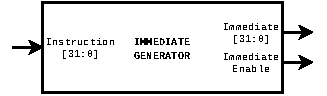
\includegraphics[scale=2]{diagrams/cpu/immgen.pdf}}
    \caption[Μονάδα Διαχείρισης Άμεσων Δεδομένων]{Η μονάδα διαχείρισης άμεσων δεδομένων}
\end{figure}
 Ανάλογα με τον τύπο της εντολής, η μονάδα μετατρέπει το κωδικοποιημένο ενσωματωμένο δεδομένο σε μήκος 32 ή 64 bit, ίσο με το μέγεθος του εντέλου του επεξεργαστή, διατηρώντας το πρόσημό του.
\vspace{1em}
\newline
\textit{Διαθέτει την εξής θύρα εισόδου:}
\begin{description}
 \item[Instruction] Θύρα εισόδου διανύσματος εντολής, μεγέθους 32 bit. \newline
 Σε αυτό το διάνυσμα βρίσκεται το κωδικοποιημένο άμεσο δεδομένο προς μετατροπή.
\end{description}
\newpage
\textit{Διαθέτει τις εξής θύρες εξόδου:}
\begin{description}
 \item[Immediate] Θύρες εξόδου αποτελέσματος της αποκωδικοποίησης και επέκτασης προσήμου, μεγέθους αντίστοιχο με αυτό του εντέλου του επεξεργαστή (32 ή 64 bit).
 \item[Immediate Enable] Θύρες εξόδου σήματος ενεργοποίησης της λειτουργίας άμεσου δεδομένου, μεγέθους ενός bit. \newline
 Ενεργοποιείται ανάλογα με τον τύπο της εντολής.
\begin{itemize} 
    \item Εάν το σήμα έχει τιμή 1, το αποτέλεσμα [Immediate] οδηγείται στην θύρα εισόδου [Β] της αριθμητικής - λογικής μονάδας.
    \item Διαφορετικά, η θύρα εισόδου [Β] της αριθμητικής - λογικής μονάδας οδηγείται από το αποτέλεσμα ανάγνωσης του καταχωρητή rs2.
\end{itemize}
\end{description}

\subsubsection{Μονάδα Διαχείρισης Διακλαδώσεων}
Η μονάδα διακλαδώσεων αναλαμβάνει τον υπολογισμό των συνθηκών με βάση τις τιμές των ορισμένων από την εντολή καταχωρητών, προκειμένου να αποφασίσει εάν θα εκτελεστεί ή όχι η επιθυμητή διακλάδωση.
Η παραπάνω λειτουργία δημιουργεί την ανάγκη για την ύπαρξη μιας θύρας αποτελέσματος της συνθήκης και δύο θύρες για την σύγκριση των δεδομένων.
Εφόσον δεν εκτελούν όλες οι εντολές κάποια διακλάδωση, υπάρχει και μια θύρα εισόδου της εντολής που ενεργοποιούν αντίστοιχα τις λειτουργίες σύγκρισης.
Άξιο αναφοράς είναι το γεγονός πως αυτή η μονάδα δεν υπολογίζει την διεύθυνση της διακλάδωσης\footnotemark, παρά μόνο αποφασίζει εάν θα πραγματοποιηθεί ή όχι.

Σχετικά με την θέση της μονάδας στην διαδικασία της διασωλήνωσης:
 \begin{itemize}
    \item Η μονάδα λειτουργεί με δεδομένα που αναγιγνώσκονται από τους καταχωρητές, άρα θα πρέπει να τοποθετηθεί \textbf{πριν το στάδιο ID}.
    \item Η λειτουργία της μονάδας είναι όμοια με την αριθμητική - λογική μονάδα επειδή και αυτή εκτελεί μια πράξη - στην συγκεκριμένη περίπτωση μια σύγκριση - σε δύο έντελα. 
    Αυτό σημαίνει ότι μπορεί να τοποθετηθεί παράλληλα με την αριθμητική - λογική μονάδα \textbf{στο στάδιο EX}.
 \end{itemize}
\footnotetext{Ο υπολογισμός της διεύθυνσης γίνεται από την αριθμητική - λογική μονάδα με την εκτέλεση της κατάλληλης πρόσθεσης, πράγμα που έχει περιγραφεί παραπάνω.}

Από τα παραπάνω, καταλήγουμε στην σχεδίαση:
\begin{figure}[H]
    \centering
    \makebox[\textwidth][c]{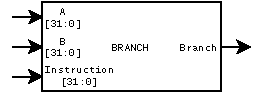
\includegraphics[scale=2]{diagrams/cpu/branch.pdf}}
    \caption[Μονάδα Διαχείρισης Διακλαδώσεων]{Η μονάδα διαχείρισης διακλαδώσεων}
\end{figure}
Η μονάδα διαχείρισης διακλαδώσεων εκτελεί την σύγκριση των δύο εντέλων που ορίζονται από την εντολή διακλάδωσης και έχει ως έξοδο ένα σήμα που υποδεικνύει εάν θα εκτελεστεί η διακλάδωση.
\vspace{1em}
\newpage
\textit{Διαθέτει τις εξής θύρες εισόδου:}
\begin{description}
 \item[Θύρα A και Θύρα B] Θύρα εισόδου εντέλου σταθερού μεγέθους, ανάλογο με το μέγεθος του εντέλου του επεξεργαστή (32 ή 64 bit). \newline
 Σε αυτές τις θύρες δίνονται οι τιμές των εντέλων για την εκτέλεση της σύγκρισης.
 \item[Instruction] Θύρα εισόδου διανύσματος εντολής, μεγέθους 32 bit. \newline
 Με βάση την τιμή του opcode του διανύσματος της εντολής αποφασίζεται η λειτουργία της σύγκρισης και γενικότερα η λειτουργία της μονάδας.
\end{description}
\textit{Διαθέτει τις εξής θύρες εξόδου:}
\begin{description}
 \item[Branch] Θύρα εξόδου σήματος διακλάδωσης, μεγέθους 1 bit.
 \begin{itemize}
     \item Εφόσον το σήμα έχει την τιμή 1, θα πρέπει να αλλάξει τιμή ο μετρητής προγράμματος, συνεπώς να γίνει εκτέλεση της διακλάδωσης.
     \item Στην τιμή 0, η μέθοδος της αλλαγής της τιμής του μετρητή προγράμματος δεν μεταβάλλεται.
 \end{itemize} 
\end{description}

\subsubsection{Μονάδα Διαχείρισης Κινδύνων}
Σκοπός αυτής της μονάδας είναι να ανιχνεύσει εντολές οι οποίες δεν θα έχουν το επιθυμητό αριθμητικό αποτέλεσμα εάν εκτελεστούν με μια συγκεκριμένη ακολουθία.
Η διαφορά στο αποτέλεσμα της εκτέλεσης συγκεκριμένων ακολουθιών εντολών οφείλεται στην τεχνική της διασωλήνωσης που εφαρμόζεται για την σχεδίαση του συγκεκριμένου μοντέλου επεξεργαστή.

Η τεχνική της διασωλήνωσης δημιουργεί κινδύνους δεδομένων σε περιπτώσεις ακολουθιών εντολών οι οποίες:
\begin{enumerate}
    \item Αρχικά, εγγράφουν το αποτέλεσμα μιας πράξης σε έναν καταχωρητή.
    \item Στην συνέχεια, αναγιγνώσκουν τον καταχωρητή με το αποτέλεσμα.
\end{enumerate}

Οι κίνδυνοι παρουσιάζονται όταν η εντολή της ανάγνωσης φτάσει στο στάδιο ID της διασωλήνωσης, όπου γίνενται ανάγνωση των καταχωρητών.
Στη σχεδίαση με την τεχνική της διασωλήνωσης ωστόσο, η εντολή όπου αποθηκεύει ένα αποτέλεσμα σε καταχωρητή μπορεί να βρίσκεται σε στάδιο προηγούμενου του WB, έχοντας ως συνέπεια να μην έχει εκτελεστεί ακόμα η λειτουργία της εγγραφής του αποτελέσματος στους καταχωρητές.
Συνεπώς, η εντολή η οποία θα αναγνώσει το περιεχόμενο του καταχωρητή, θα συνεχίσει την εκτέλεσή της με την προηγούμενη τιμή, και όχι με το αποτέλεσμα της προηγούμενης εντολής όπως θα ήταν αναμενόμενο από την ακολουθιακή εκτέλεση των δύο αυτών εντολών. \newline

Σχετικά με την θέση της μονάδας στην διαδικασία της διασωλήνωσης:
 \begin{itemize}
    \item Αξιοποιεί το διάνυσμα της εντολής προς εκτέλεση, συνεπώς θα πρέπει να τοποθετηθεί \textbf{μετά το στάδιο IF}.
    \item Η μονάδα ελέγχει ποιες εντολές θα προχωρήσουν με την λειτουργία ανάγνωσης καταχωρητών, άρα θα πρέπει να βρίσκεται \textbf{προτού το στάδιο ID}.
    \item Εφόσον δεν ορίζεται κάποιο στάδιο πριν το IF και μετά το ID, θα πρέπει να οριστεί ένα \textbf{νέο στάδιο ανάμεσα στο IF και στο ID}, το οποίο θα ονομάζουμε \textbf{στάδιο ΗΑΖ} (Hazard).
 \end{itemize}
\newpage
Καταλήγουμε στην παρακάτω σχεδίαση της μονάδας διαχείρισης κινδύνων:
\begin{figure}[H]
    \centering
    \makebox[\textwidth][c]{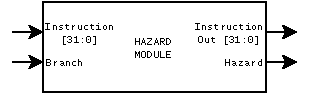
\includegraphics[scale=2]{diagrams/cpu/hazard.pdf}}
    \caption[Μονάδα Διαχείρισης Κινδύνων]{Η μονάδα διαχείρισης κινδύνων}
\end{figure}
Η μονάδα αυτή ανιχνεύει τους καταχωρητές που πρόκειται να χρησιμοποιήσει κάθε εντολή και με βάση αυτούς παύει την εκτέλεση της επόμενης εντολής, εφόσον προκαλεί κίνδυνο δεδομένου.
 Μια τέτοια μονάδα θα μπορούσε να παραλειφθεί, αφήνοντας την διαχείριση τέτοιων προβλημάτων στον Assembler ή στον προγραμματιστή\footnotemark.
 \footnotetext{Η αρχιτεκτονική RISC-V δεν αναφέρει καμία ακολουθία εντολών προς αποφυγή, άρα οποιοσδήποτε κίνδυνος προκύπτει θα πρέπει να αντιμετωπίζεται σε επίπεδο υλικού, έτσι ώστε να εκτελούνται με τα ορισμένα από τις προδιαγραφές αποτελέσματα. }
\vspace{1em}
\newline
\textit{Διαθέτει τις εξής θύρες εισόδου:}
\begin{description}
 \item[Instruction] Θύρα εισόδου διανύσματος εντολής, μεγέθους 32 bit.
 \item[Branch] Θύρα εισόδου σήματος διακλάδωσης του ενός bit. \newline
 Σε περίπτωση που πρόκεται να γίνει διακλάδωση, το διάνυσμα στην έξοδο εντολής της μονάδας γίνεται 0, για να αποφευχθεί η εκτέλεση του λάθος τμήματος του προγράμματος.
\end{description}
\textit{Διαθέτει τις εξής θύρες εξόδου:}
\begin{description}
 \item[Hazard] Θύρα εξόδου σήματος ύπαρξης Hazard, μεγέθους 1 bit.
 \begin{itemize}
     \item Εφόσον το σήμα έχει την τιμή 1, ο μετρητής προγράμματος δεν μεταβάλλει την τιμή του, αφήνοντας έναν κύκλο ρολογιού πριν προχωρήσει στην επόμενη εντολή.
     Πρακτικά, δημιουργείται ένα Pipeline Bubble.
     \item Στην τιμή 0, η μέθοδος της αλλαγής της τιμής του μετρητή προγράμματος δεν μεταβάλλεται.
 \end{itemize} 
 \item[Instruction Out] Θύρες εξόδου διανύσματος εντολής, μεγέθους 32 bit. \newline
 Η εντολή που βρίσεται σε αυτή την θύρα προωθείται στις μονάδες των επόμενων σταδίων διασωλήνωσης προς εκτέλεση.
\end{description}


\subsection{Τελικό Μοντέλο - Ένα Απλό RISC-V RV(32/64)I Hardware Thread}
Συνδυάζοντας την τεχνική της διασωλήνωσης, τις παραπάνω μονάδες και τις εντολές που βρίσκονται στο σύνολο RV32I μπορούμε να οδηγηθούμε στην οργάνωση των σταδίων της διασωλήνωσης και στην λεπτομερέστερη διασύνδεση των λειτουργικών μονάδων.
Η διασύνδεση θα χρειαστεί να αξιοποιήσει περαιτέρω στοιχεία λογικού σχεδιασμού για να καταφέρει να αποτελεί μια ολοκληρωμένη, λειτουργική σχεδίαση.
\newpage
Οι σχεδιαστικές αποφάσεις στο επίπεδο της μικροαρχιτεκτονικής είναι οι εξής:
\begin{itemize}
    \item Η τεχνική της διασωλήνωσης απαιτεί κάθε στάδιο να εκτελεί διαφορετική εντολή, με τα στάδια να τροφοδοτούν το επόμενό τους.
    Η πρόταση αυτή ορίζει καταχωρητές οι οποίοι θα ολισθαίνουν το διάνυσμα της εντολής από το ένα στάδιο στο επόμενο.
    Στην συγκεκριμένη σχεδίαση, οι καταχωρητές αυτοί χρησιμοποιούν την ονοματολογία με \textbf{πρόθεμα} \texttt{\textbf{P\_}}.
    \item Λόγω της διασωλήνωσης ορίζουμε επίσης καταχωρητές οι οποίοι αποθηκεύουν την τιμή του μετρητή προγράμματος για την εντολή που εκτελεί κάθε στάδιο, με την ονοματολογία με \textbf{πρόθεμα} \texttt{\textbf{PC\_}}.
    \item Τα σταθερά πεδία κωδικοποιήσεων επιβάλλουν την σταθερή διασύνδεση των πεδίων του διανύσματος της εντολής με τις αντίστοιχες λειτουργικές μονάδες.
    \item Η απουσία μικροκώδικα και μονάδας ελέγχου για την οργάνωση των υπολειτουργιών λύνεται με την αποκωδικοποίηση του πεδίου \texttt{opcode} σε κάθε στάδιο της διασωλήνωσης από τις λειτουργικές μονάδες.
    \item Ο αποκλεισμός των αχρησιμοποίητων πεδίων κάθε κωδικοποίησης γίνεται με την χρήση πολυπλεκτών και με σήματα ελέγχου που παράγονται ή αναγιγνώσκονται από τις μονάδες.
\end{itemize}
Οι σχεδιαστικές αποφάσεις στο επίπεδο της διασύνδεσης των μονάδων είναι οι εξής:
\begin{itemize}
    \item Οι εντολές πράξεων χωρίζονται σε εντολές πράξεων καταχωρητή - καταχωρητή και καταχωρητή - άμεσου δεδομένου.
    Η ειδοποιός διαφορά των εντολών καταχωρητή - καταχωρητή και καταχωρητή - άμεσου δεδομένου βρίσκεται στην αντικατάσταση ή όχι του πεδίου \texttt{rs2} με το πεδίο \texttt{imm}, ενώ το πεδίο \texttt{rs1} παραμένει ως έχει.
    Η μονάδα διαχείρισης άμεσων δεδομένων διαθέτει σήμα ενεργοποίησης για τις εντολές που χρησιμοποιούν άμεσο δεδομένο.
    Από τα παραπάνω οδηγούμαστε στην τοποθέτηση ενός πολυπλέκτη για τον καθορισμό της εισόδου \texttt{B} της αριθμητικής - λογικής μονάδας, με σήμα επιλογής την έξοδο \texttt{Immediate Enable}, για την επιλογή του καταχωρητή \texttt{rs2} ή του άμεσου δεδομένου \texttt{imm} αντίστοιχα.
    \item Για την εκτέλεση των εντολών διακλάδωσης και της εντολής \texttt{auipc}, χρειάζεται να υπολογιστεί η πρόσθεση ενός άμεσου δεδομένου με την τιμή του μετρητή προγράμματος της εντολής.
    Σκοπός του πολυπλέκτη στην είσοδο \texttt{A} της αριθμητικής - λογικής μονάδας είναι να ενεργοποιεί την είσοδο του δεδομένου της τιμής του μετρητή προγράμματος, εντοπίζοντας τέτοιου τύπου εντολές από το πεδίο \texttt{opcode} του καταχωρητή \texttt{P\_ID}.
    \item Ο καταχωρητής \texttt{rs2\_dmem} χρησιμοποιείται για να αποθηκεύσει στο στάδιο EX, το δεδομένο που αναγνώστηκε από τον δεύτερο καταχωρητή προς ανάγνωση από το αρχείο καταχωρητών.
    Το δεδομένο προχωράει στην κατάλληλη θύρα της μνήμης δεδομένων για εγγραφή του, εφόσον η εντολή είναι τύπου Store.
    \item Ο καταχωρητής \texttt{res\_wb} χρησιμοποιείται για να αποθηκεύσει στο στάδιο MEM/WB το αποτέλεσμα της αριθμητικής πράξης το οποίο θα εγγραφεί στον καταχωρητή που ορίζει το πεδίο \texttt{rd}.
    \newpage
    \item Ορίζεται ένας πολυπλέκτης για την επιλογή του δεδομένου προς εγγραφή στον καταχωρητή που ορίζει το πεδίο \texttt{rd}.
    Πιο συγκεκριμένα, η επιλογή της πηγής του δεδομένου προς εγγραφή ορίζεται από τον τύπο της εντολής, άρα από το πεδίο \texttt{opcode} του καταχωρητή \texttt{P\_MEM}.
    Υπάρχουν 4 πηγές δεδομένων προς εγγραφή στον καταχωρητή που ορίζει το πεδίο \texttt{rd}:
    \begin{itemize}
        \item Οι \textbf{εντολές αριθμητικών πράξεων} χρειάζεται να εγγράψουν στον καταχωρητή που ορίζει το πεδίο \texttt{rd} το περιεχόμενο του καταχωρητή αποτελέσματος \texttt{res\_wb}.
        \item Οι \textbf{εντολές φόρτωσης} χρειάζεται να εγγράψουν στον καταχωρητή που ορίζει το πεδίο \texttt{rd} το δεδομένο που αναγιγνώσκεται από την θύρα \texttt{rs} (θύρα εισόδου / εξόδου \texttt{Data}) της μνήμης δεδομένων.
        \item Η \textbf{εντολή φόρτωσης άμεσου δεδομένου} \texttt{lui} έχει υλοποιηθεί έτσι ώστε να φορτώνεται από το περιεχόμενο του καταχωρητή \texttt{P\_MEM}.
        Δεν έχει οριστεί ειδική πράξη στην αριθμητική - λογική μονάδα για τον υπολογισμό του ορθού αποτελέσματος και εγγραφή του μέσω του καταχωρητή \texttt{res\_wb}, όπως τις παραπάνω πράξεις, γι αυτό χρησιμοποιείται κατευθείαν ο παραπάνω καταχωρητής.
        \item Οι \textbf{εντολές άλματος} αποθηκεύουν την τρέχουσα τιμή του μετρητή προγράμματος στον καταχωρητή που ορίζει το πεδίο \texttt{rd}.
        Συνεπώς, πηγή του δεδομένου προς εγγραφή είναι επίσης ο καταχωρητής \texttt{PC\_MEM}.
    \end{itemize}
    \item Οι εντολές βρόχου και άλματος τροποποιούν το περιεχόμενο του μετρητή προγράμματος, όπου στο συγκεκριμένο διάγραμμα μικροαρχιτεκτονικής αναφέρεται ως \texttt{PC}.
    \begin{itemize}
        \item Σε περίπτωση που δεν υπάρχει αλλαγή από τέτοιου τύπου εντολές, η τιμή του μετρητή προγράμματος αυξάνεται κατά 4 έτσι ώστε να δεικτοδοτεί την επόμενη εντολή προς εκτέλεση.
        \item Εάν αποφασιστεί από την μονάδα διαχείρισης διακλαδώσεων πως θα πρέπει να αλλάξει η ροή του προγράμματος, θα πρέπει να εγγραφεί στον μετρητή προγράμματος η τιμή του αποτελέσματος της πρόσθεσης που θα εκτελέσει η αριθμητική - λογική μονάδα.
        \item Σε περίπτωση που υπάρχει κίνδυνος δεδομένου, ο μετρητής προγράμματος θα πρέπει να διατηρήσει την τιμή του αμετάβλητη, έχοντας ως αποτέλεσμα μια προσωρινή παύση της εκτέλεσης νέων εντολών από τον επεξεργαστή.
    \end{itemize}
    Τα σήματα που οδηγούν τον πολυπλέκτη του μετρητή προγράμματος είναι τα σήματα \texttt{br (Branch)} και \texttt{hz (Hazard)}, που παράγουν οι μονάδες διαχείρισης διακλαδώσεων και κινδύνων αντίστοιχα.
\end{itemize}

Οι περιγραφές των λειτουργικών μονάδων στις παραπάνω υποενότητες σε συνδυασμό με τις περιγραφές των προδιαγραφών \cite{spec} για την εκτέλεση των εντολών στο σύνολο RV32I οδηγούν στην παρακάτω μικροαρχιτεκτονική:
\begin{sidewaysfigure}
    \centering
    \makebox[\textwidth][c]{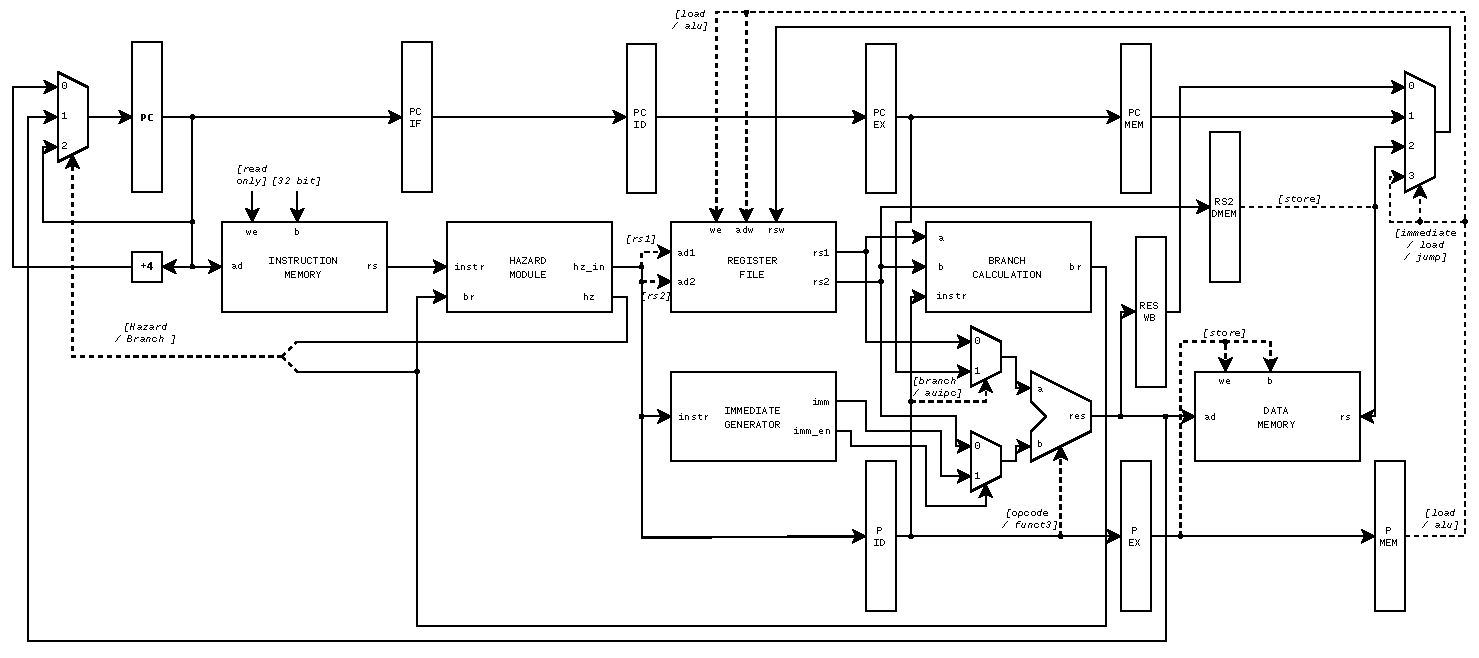
\includegraphics[width=\textwidth]{diagrams/cpu/arch.pdf}}
    \caption{Τελική μικροαρχιτεκτονική του επεξεργαστή}
\end{sidewaysfigure}

\newpage
\subsection{Επεκτασιμότητα του μοντέλου}
Προαναφέρεται πως ορισμένες μονάδες παρέχουν υποστήριξη για μεταβλητό μέγεθος εντέλου για την εκτέλεση των λειτουργιών τους.
Με μια παραμετροποίηση των μεγεθών των καταχωρητών δεδομένων των μονάδων και με επέκταση των λειτουργιών της μνήμης δίνεται η δυνατότητα επιλογής της υποστηριζόμενης αρχιτεκτονικής συνόλου εντολών.
Το βασικό μοντέλο παρέχει υποστήριξη για 2 αρχιτεκτονικές συνόλου εντολών χωρίς καμία αλλαγή στην μικροαρχιτεκτονική:
\begin{itemize}
    \item Μέγεθος εντέλου 32-bit, συνεπώς υποστήριξη αρχιτεκτονικής συνόλου εντολών RV32I.
    \item Μέγεθος εντέλου 64-bit, συνεπώς υποστήριξη αρχιτεκτονικής συνόλου εντολών RV64I.
\end{itemize}
\subsection{Ενδεικτική σύνθεση της περιγραφής του επεξεργαστή}
Εκτελέστηκε μια διαδικασία σύνθεσης των περιγραφών του υλικού του επεξεργαστή σε FPGA.
Σκοπός της διαδικασίας σύνθεσης ήταν η απόδειξη της υλοποιησιμότητας του μοντέλου σε έναν βασικό βαθμό.

Οι περιγραφές υλικού αποδείχθηκαν συνθέσιμες, χωρίς ωστόσο να ελεγχθούν μετά την σύνθεσή τους για την ορθότητα της λειτουργικότητας του σχεδιασμού.
Ο θεωρητικός σχεδιασμός είναι απολύτως λειτουργικός, έχοντας τα αναμενόμενα από τις προδιαγραφές αποτελέσματα μετά την εκτέλεση εντολών και ακολουθιών εντολών. 

Για την σύνθεση χρειάστηκε να οριστούν θύρες εισόδου και εξόδου στο μοντέλο του επεξεργαστή, έτσι ώστε να μην απλοποιηθεί σε βαθμό κατακερματισμού από την διαδικασία της σύνθεσης.
Αποφασίστηκε πως ο υλοποιήσιμος μικροεπεξεργαστής θα δέχεται ως είσοδο ένα σήμα ρολογιού και ως έξοδο θα εκθέτει τα σήματα αποτελέσματος της αριθμητικής - λογικής μονάδας \texttt{res} και την θύρα δεδομένων της μνήμης δεδομένων \texttt{rs}, για προσομοίωση μιας απλής διεπαφής με μία εξωτερική μνήμη δεδομένων.
Επιλέχθηκαν επίσης αρκετά μικρά μεγέθη μνημών δεδομένων και εντολών, έτσι ώστε να εξαλειφθεί τυχούσα υπερκάλυψη των μονάδων (μπλοκ) του FPGA.

Αξιοποιούνται τα αναμενόμενα μπλοκ ειδικού σκοπού του FPGA για την υλοποίηση της αριθμητικής - λογικής μονάδας, του αρχείου καταχωρητών, τις μνήμες εντολών και δεδομένων.
Οι υπόλοιπες μονάδες συντέθηκαν από μπλοκ γενικού σκοπού του FPGA.
Η σύνθεση είχε ως αποτέλεσμα χρονισμού ρολόι με συχνότητα 148 MHz, χωρίς καμία βελτιστοποίηση, αφού οι περιγραφές υλικού δεν έχουν σχεδιαστεί με γνώμονα την διαδικασία της σύνθεσης.


\section{ΕΛΕΓΧΟΣ ΛΕΙΤΟΥΡΓΙΩΝ - ΚΥΜΑΤΟΜΟΡΦΕΣ}
\subsection{Μονάδα Μνήμης}
Η μονάδα μνήμης αρχικοποιείται με υποστήριξη για τις εντολές RV64I, έτσι ώστε να αναδειχθούν όλες οι λειτουργίες της.
Φορτώνεται με δεδομένα από το αρχείο \texttt{memtest.mem}, κατ' αυτόν τον τρόπο:
\begin{table}[H]
    \makebox[\textwidth][c]{
    \begin{tabular}{|r|l|} 
        \hline
        \cellcolor{lgray} \textbf{Θέση Μνήμης} & \cellcolor{lgray} \textbf{Περιεχόμενο} \\\hline
        \texttt{0x0000} & \texttt{00 11 22 33} \\\hline
        \texttt{0x0004} & \texttt{44 55 66 77} \\\hline
        \texttt{0x0008} & \texttt{88 99 aa bb} \\\hline
        \texttt{0x000A} & \texttt{cc dd ee ff} \\\hline
        \texttt{0x0010} & \texttt{01 23 45 67} \\\hline
    \end{tabular} }
\end{table}
Παραδείγματα λειτουργιών:
\begin{figure}[H]
\renewcommand{\figurename}{Κυματομορφή} 
\centering
\makebox[\textwidth][c]{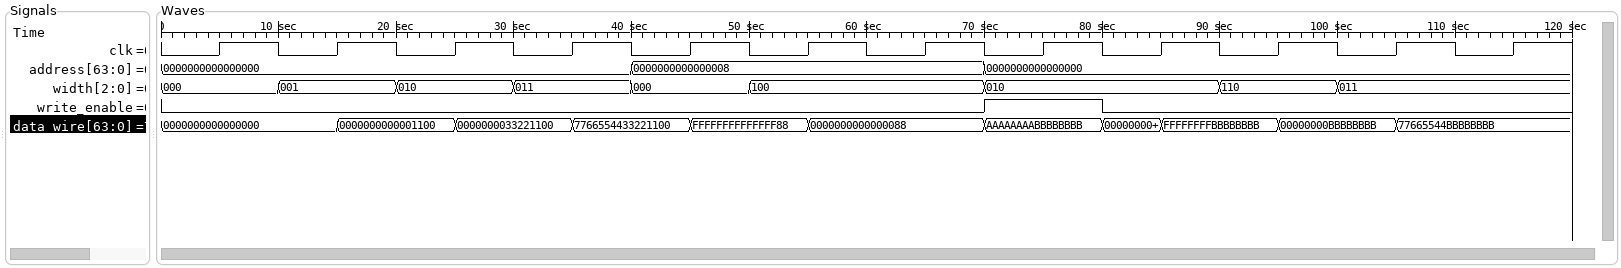
\includegraphics[width=1.3\textwidth]{diagrams/wave/memtest.png}}
\caption[Κυματομορφή - Μονάδα Μνήμης]{Κυματομορφή Λειτουργιών της Μονάδας Μνήμης.}
\end{figure}
\begin{description}
\item[Χρονική στιγμή 0] \hfill \newline 
Προετοιμασία ανάγνωσης ενός byte στην θέση μνήμης με διεύθυνση \texttt{0x0000} και επέκταση προσήμου.
\begin{itemize}
    \item Σήμα εισόδου \texttt{address} \newline Ορισμός διεύθυνσης προσπέλασης στην θέση \texttt{0x0000}.
    \item Σήμα εισόδου \texttt{width} \newline Ορισμός μεγέθους προσπέλασης στην τιμή \texttt{000}, άρα 1 byte με επέκταση προσήμου.
    \item Σήμα εισόδου \texttt{write\textunderscore enable} \newline Ορισμός σήματος εγγραφής στην τιμή \texttt{0}, άρα λειτουργία ανάγνωσης.
\end{itemize}
\item[Χρονική στιγμή 5]\hfill \newline 
Αποτέλεσμα ανάγνωσης ενός byte στην θέση \texttt{0x0000} με επέκταση προσήμου.
\begin{itemize}
    \item Σήμα εξόδου \texttt{data\_wire} \newline Από την μνήμη διαβάζεται το περιεχόμενο \texttt{0x00} της θέσης \texttt{0x0000}, με επέκταση προσήμου.
\end{itemize}
\item[Χρονική στιγμή 10] \hfill \newline
Προετοιμασία ανάγνωσης δύο byte στην θέση \texttt{0x0000} και επέκταση προσήμου.
\begin{itemize}
    \item Σήμα εισόδου \texttt{width} \newline Ορισμός μεγέθους προσπέλασης στην τιμή \texttt{001}, άρα 2 byte με επέκταση προσήμου.
    \item Άλλα σήματα εισόδου \newline Παραμένουν ως έχουν.
\end{itemize}
\newpage
\item[Χρονική στιγμή 15] \hfill \newline
Αποτέλεσμα ανάγνωσης δύο byte στην θέση \texttt{0x0000} με επέκταση προσήμου.
\begin{itemize}
    \item Σήμα εξόδου \texttt{data\_wire} \newline Από την μνήμη διαβάζεται το περιεχόμενο \texttt{0x1100} της θέσης \texttt{0x0000}, με επέκταση προσήμου.
\end{itemize}
\item[Χρονικές στιγμές 20, 25, 30, 35] \hfill \newline
Διαδοχικές αναγνώσεις της θέσης μνήμης \texttt{0x0000} και αποτελέσματά τους με επαύξηση μεγέθους ανάγνωσης στα 4 και 8 byte αντίστοιχα, με επέκταση προσήμου. \newline
Ακολουθείται η ίδια διαδικασία αλλάζοντας μόνο το σήμα \texttt{width}, με τα αντίστοιχα αποτελέσματα.
\item [Χρονική στιγμή 40] \hfill \newline
Προετοιμασία ανάγνωσης ενός byte στην θέση \texttt{0x0008} και επέκταση προσήμου με εφαρμογή των αντίστοιχων σημάτων.
\item [Χρονική στιγμή 45] \hfill \newline
Αποτέλεσμα ανάγνωσης του byte στην θέση \texttt{0x0000} με επέκταση προσήμου.
\item [Χρονική στιγμή 50] \hfill \newline
Προετοιμασία ανάγνωσης ενός byte στην θέση \texttt{0x0008} χωρίς επέκταση προσήμου.
\begin{itemize}
    \item Σήμα εισόδου \texttt{width} \newline Ορισμός μεγέθους προσπέλασης στην τιμή \texttt{100}, άρα 1 byte χωρίς επέκταση προσήμου.
    \item Άλλα σήματα εισόδου \newline Παραμένουν ως έχουν.
\end{itemize}
\item [Χρονική στιγμή 55] \hfill \newline
Αποτέλεσμα ανάγνωσης του byte στην θέση \texttt{0x0008} χωρίς επέκταση προσήμου.
\item [Χρονική στιγμή 70] \hfill \newline
Προετοιμασία για εγγραφή του δεδομένου \texttt{0xAAAAAAAABBBBBBBB} στην διεύθυνση μνήμης \texttt{0x0000}.
\begin{itemize}
    \item Σήμα εισόδου \texttt{address} \newline Ορισμός διεύθυνσης προσπέλασης στην θέση \texttt{0x0000}.
    \item Σήμα εισόδου \texttt{width} \newline Ορισμός μεγέθους προσπέλασης στην τιμή \texttt{010}, άρα 4 byte.
    \item Σήμα εισόδου \texttt{write\textunderscore enable} \newline Ορισμός σήματος εγγραφής στην τιμή \texttt{1}, άρα λειτουργία εγγραφής.
    \item Σήμα εισόδου \texttt{data\textunderscore enable} \newline Ορισμός του δεδομένου \texttt{0xAAAAAAAABBBBBBBB} προς εγγραφή.
\end{itemize}
\item [Χρονική στιγμή 80] \hfill \newline
Προετοιμασία ανάγνωσης 4 byte στην θέση \texttt{0x0000} και επέκταση προσήμου, με εφαρμογή των αντίστοιχων σημάτων.
\item [Χρονική στιγμή 85] \hfill \newline
Αποτέλεσμα ανάγνωσης 4 byte στην θέση \texttt{0x0000} με επέκταση προσήμου.
\item [Χρονική στιγμή 90] \hfill \newline
Προετοιμασία ανάγνωσης 4 byte στην θέση \texttt{0x0000} χωρίς επέκταση προσήμου, με εφαρμογή των αντίστοιχων σημάτων.
\item [Χρονική στιγμή 95] \hfill \newline
Αποτέλεσμα ανάγνωσης 4 byte στην θέση \texttt{0x0000} χωρίς επέκταση προσήμου.
\item [Χρονική στιγμή 100] \hfill \newline
Προετοιμασία ανάγνωσης 8 byte στην θέση \texttt{0x0000}, με εφαρμογή των αντίστοιχων σημάτων.
\item [Χρονική στιγμή 105] \hfill \newline
Αποτέλεσμα ανάγνωσης 8 byte στην θέση \texttt{0x0000}.
\end{description}

\subsection{Αριθμητική - Λογική Μονάδα}
Παραδείγματα λειτουργιών:
\begin{figure}[H]
\renewcommand{\figurename}{Κυματομορφή} 
\centering
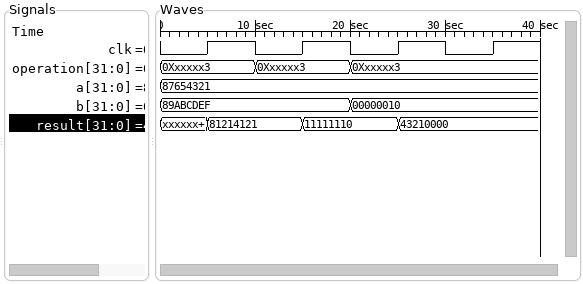
\includegraphics[scale=0.6]{diagrams/wave/alutest.png}
\caption[Κυματομορφή - Αριθμητική - Λογική Μονάδα]{Κυματομορφή λειτουργιών της Αριθμητικής - Λογικής μονάδας.}
\end{figure}
\begin{description}
\item[Χρονική στιγμή 0] \hfill \newline
Προετοιμασία των σημάτων εισόδου για εκτέλεση της λογικής πράξης AND ως εξής:
\begin{itemize}
    \item Σήμα εισόδου \texttt{Α} \newline Ορισμός δεδομένου Α ως \texttt{0x87654321}.
    \item Σήμα εισόδου \texttt{Β} \newline Ορισμός δεδομένου B ως \texttt{0x89ABCDEF}.
    \item Σήμα εισόδου \texttt{Operation} \newline Ορισμός της πράξης προς εκτέλεση ως λογικό AND, με αδιάφορη τιμή x στα bit που δεν επηρεάζουν τον ορισμό της πράξης.
\end{itemize}
\item[Χρονική στιγμή 5] \hfill \newline
Αποτέλεσμα της πράξης \texttt{0x87654321 \textampersand\space 0x89ABCDEF} που είναι \texttt{0x81214121}.
\item[Χρονική στιγμή 10] \hfill \newline
Προετοιμασία του σήματος εισόδου \texttt{Operation} για την εκτέλεση της αριθμητικής πράξης ADD. Η υπερχείλιση αγνοείται.
\item[Χρονική στιγμή 15] \hfill \newline
Αποτέλεσμα της πράξης \texttt{0x87654321 + 0x89ABCDEF} το οποίο είναι \texttt{0x11111110}.
\newpage
\item[Χρονική στιγμή 20] \hfill \newline
Προετοιμασία των σημάτων εισόδου για εκτέλεση της λογικής πράξης αριστερής ολίσθησης (εντολή sll) ως εξής:
\begin{itemize}
    \item Σήμα εισόδου \texttt{A} \newline Ορισμός δεδομένου A ως \texttt{0x87654321}.
    \item Σήμα εισόδου \texttt{B} \newline Ορισμός δεδομένου B ως \texttt{0x00000010}, για ολίσθηση της εισόδου A κατά 4.
    \item Σήμα εισόδου \texttt{Operation} \newline Ορισμός της πράξης προς εκτέλεση ως αριστερή ολίσθηση, με αδιάφορη τιμή x στα bit που δεν επηρεάζουν τον ορισμό της πράξης.
\end{itemize}
\item[Χρονική στιγμή 25] \hfill \newline
Αποτέλεσμα της πράξης \texttt{0x87654321 \textless\textless\space 4} το οποίο είναι \texttt{0x43210000}.
\end{description}

\subsection{Αρχείο Καταχωρητών}
Παραδείγματα λειτουργιών:
\begin{figure}[H]
\centering
\renewcommand{\figurename}{Κυματομορφή} 
\makebox[\textwidth][c]{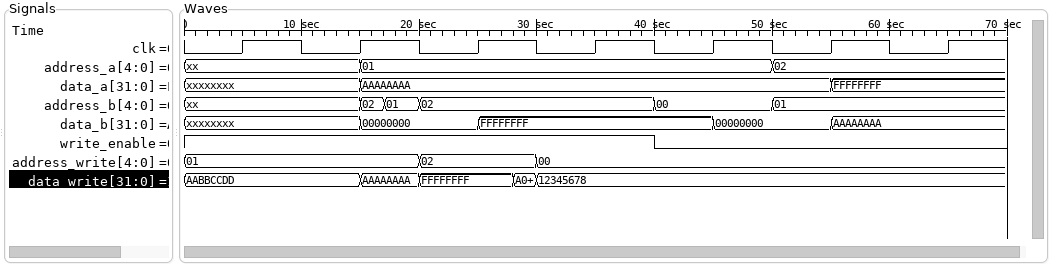
\includegraphics[width=1.2\textwidth]{diagrams/wave/regtest.png}}
\caption[Κυματομορφή - Αρχείο Καταχωρητών]{Κυματομορφή λειτουργιών του Αρχείου Καταχωρητών.}
\end{figure}
\begin{description}
\item[Χρονική στιγμή 0] \hfill \newline
Προετοιμασία των σημάτων εισόδου για εγγραφή δεδομένου σε καταχωρητή.
\begin{itemize}
    \item Σήμα εισόδου \texttt{address\_write} \newline Ορισμός διεύθυνσης καταχωρητή προς εγγραφή ως \texttt{0x01}.
    \item Σήμα εισόδου \texttt{data\_write} \newline Ορισμός δεδομένου προς εγγραφή ως \texttt{0xAABBCCDD}.
    \item Σήμα εισόδου \texttt{write\_enable} \newline Ορισμός σήματος εγγραφής στην τιμή \texttt{1}, έτσι ώστε να πραγματοποιηθεί η εγγραφή του δεδομένου στον ορισμένο καταχωρητή.
\end{itemize}
\item[Χρονική στιγμή 5] \hfill \newline
Εγγραφή του δεδομένου \texttt{0xAABBCCDD} στον καταχωρητή με διεύθυνση \texttt{0x01}.
\newpage
\item[Χρονική στιγμή 15] \hfill \newline
Προετοιμασία των σημάτων εισόδου για εγγραφή δεδομένου σε καταχωρητή και αναγνώσεις δύο καταχωρητών.
\begin{itemize}
    \item Σήμα εισόδου \texttt{address\_write} \newline Ορισμός διεύθυνσης καταχωρητή προς εγγραφή ως \texttt{0x01}.
    \item Σήμα εισόδου \texttt{data\_write} \newline Ορισμός δεδομένου προς εγγραφή ως \texttt{0xAAAAAAAA}.
    \item Σήμα εισόδου \texttt{write\_enable} \newline Ορισμός σήματος εγγραφής στην τιμή \texttt{1}, έτσι ώστε να πραγματοποιηθεί η εγγραφή του δεδομένου στον ορισμένο καταχωρητή.
    \item Σήμα εισόδου \texttt{address\_a} \newline Ορισμός διεύθυνσης πρώτου καταχωρητή προς ανάγνωση ως \texttt{0x01}.
    \item Σήμα εισόδου \texttt{address\_b} \newline Ορισμός διεύθυνσης δεύτερου καταχωρητή προς ανάγνωση ως \texttt{0x02}.
\end{itemize}
Ταυτόχρονα, παρατηρείται στα σήματα εξόδου:
\begin{itemize}
    \item Σήμα εξόδου \texttt{data\_a} \newline Ανάγνωση της τιμής \texttt{0xAAAAAAAA} από τον καταχωρητή με διεύθυνση \texttt{0x01}.
    Στον συγκεκριμένο καταχωρητή συμβαίνει αυτή την στιγμή η εγγραφή του δεδομένου \texttt{0xAAAAAAAA}, το οποίο διαβάζουμε.
    Σε περίπτωση που οι λειτουργίες εγγραφής και ανάγνωσης δεν υποστηρίζονταν ταυτόχρονα στον ίδιο καταχωρητή, θα αναγιγνωσκόταν το δεδομένο \texttt{0xAABBCCDD} που βρισκόταν μέχρι πρότινος στον καταχωρητή με διεύθυνση \texttt{0x01}.
    \item Σήμα εξόδου \texttt{data\_b} \newline Ανάγνωση της τιμής \texttt{0x00000000} από τον καταχωρητή με διεύθυνση \texttt{0x02}.
\end{itemize}
\item[Χρονική στιγμή 17] \hfill \newline
Απρόσμενη μεταβολή του σήματος εισόδου \texttt{address\_b} το οποίο δεν αλλάζει την τρέχουσα τιμή που είχε αναγνωστεί στην θετική ακμή του ρολογιού, την στιγμή 15.
\item[Χρονική στιγμή 20] \hfill \newline
Προετοιμασία των σημάτων εισόδου που αφορούν την λειτουργία εγγραφής, έτσι ώστε να εγγραφεί το δεδομένο \texttt{0xFFFFFFFF} στον καταχωρητή με διεύθυνση \texttt{0x02}.
\item[Χρονική στιγμή 25] \hfill \newline
Ταυτόχρονη λειτουργία εγγραφής και ανάγνωσης του δεδομένου \texttt{0xFFFFFFFF} που αφορά τον καταχωρητή με διεύθυνση \texttt{0x02}.
\item[Χρονική στιγμή 28] \hfill \newline
Απρόσμενη μεταβολή του σήματος εισόδου \texttt{data\_write} το οποίο δεν αλλάζει την προηγούμενη τιμή εγγραφής στην θετική ακμή του ρολογιού, την στιγμή 25.
\item[Χρονική στιγμή 30] \hfill \newline
Προετοιμασία των σημάτων εισόδου που αφορούν την λειτουργία εγγραφής, έτσι ώστε να εγγραφεί το δεδομένο \texttt{0x12345678} στον καταχωρητή με διεύθυνση \texttt{0x00}.
\item[Χρονική στιγμή 35] \hfill \newline
Εγγραφή του δεδομένου \texttt{ox12345678} στον καταχωρητή με διεύθυνση \texttt{0x00}.
\item[Χρονική στιγμή 40] \hfill \newline
Προετοιμασία σημάτων εισόδου για ανάγνωση των περιεχομένων των καταχωρητών των διευθύνσεων \texttt{0x01} και \texttt{0x00}.
\item[Χρονική στιγμή 45] \hfill \newline
Ανάγνωση των τιμών των καταχωρητών με διευθύνσεις\texttt{0x01} και \texttt{0x00}.
Παρατηρείται ότι παρά την εγγραφή του δεδομένου \texttt{0x12345678} στον καταχωρητή με διεύθυνση \texttt{0x00}, η ανάγνωσή του επιστρέφει σταθερά την τιμή \texttt{0x00000000}, όπως ορίζεται από τις προδιαγραφές \cite{spec}.
\end{description}

\subsection{Μονάδα Διαχείρισης Άμεσων Δεδομένων}
Παραδείγματα Λειτουργιών:
\begin{figure}[H]
\centering
\renewcommand{\figurename}{Κυματομορφή} 
\makebox[\textwidth][c]{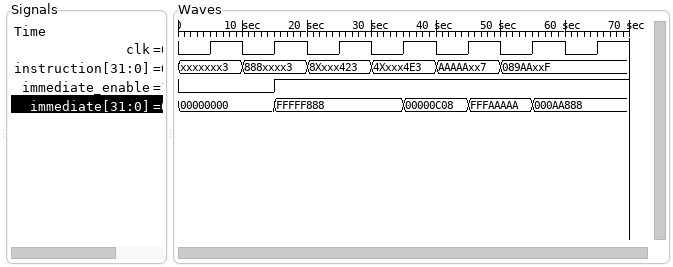
\includegraphics[scale=0.5]{diagrams/wave/immtest.png}}
\caption[Κυματομορφή - Μονάδα Διαχείρισης Άμεσων Δεδομένων]{Κυματομορφή λειτουργιών της μονάδας Διαχείρισης Άμεσων Δεδομένων}
\end{figure}
\begin{description}
\item[Χρονική στιγμή 0] \hfill \newline
Προετοιμασία σήματος εισόδου διανύσματος εντολής τύπου R για αποκωδικοποίηση, με αδιάφορη τιμή x στα bit που δεν επηρεάζουν την λειτουργία της μονάδας.
\item[Χρονική στιγμή 5] \hfill \newline
Αποτέλεσμα αποκωδικοποίησης άμεσου δεδομένου.
Στις εντολές τύπου R δεν υπάρχει άμεσο δεδομένο και το σήμα ενεργοποίησης παίρνει την τιμή \texttt{0}.
\item[Χρονική στιγμή 10] \hfill \newline
Προετοιμασία σήματος εισόδου διανύσματος εντολής τύπου I για αποκωδικοποίηση, με αδιάφορη τιμή x στα bit που δεν επηρεάζουν την λειτουργία της μονάδας.
Το διάνυσμα κωδικοποιεί το άμεσο δεδομένο \texttt{0x888}.
\item[Χρονική στιγμή 15] \hfill \newline
Αποτέλεσμα αποκωδικοποίησης του άμεσου δεδομένου \texttt{0x888}.
Με την απαραίτητη επέκταση προσήμου η αποκωδικοποίηση παίρνει την τιμή \texttt{0xFFFFF888} και επιπλέον το σήμα ενεργοποίησης παίρνει την τιμή \texttt{1}.
\item[Χρονικές στιγμές 20, 25, 30, 35, 40, 45, 50, 55] \hfill \newline
Προετοιμασία του σήματος εισόδου διανυσμάτων εντολών τύπου S, B, U, J και αποτελέσματά τους αντίστοιχα.
Το σήμα ενεργοποίησης παίρνει την τιμή 1 για κάθε μία από τις παρακάτω κωδικοποιήσεις εντολών, καθώς κωδικοποιούν άμεσο δεδομένο.\newline
Κωδικοποιούνται με την σειρά οι αριθμοί:
\begin{itemize}
    \item \texttt{0x888} στην κωδικοποίηση S - type, όπου με επέκταση προσήμου παράγει το αποτέλεσμα \texttt{0xFFFFF888}.
    \item \texttt{0x0C08} στην κωδικοποίηση B - type, όπου με επέκταση προσήμου παράγει το αποτέλεσμα \texttt{0x00000C08}.
    \item \texttt{0xAAAAA} στην κωδικοποίηση U - type, όπου με επέκταση προσήμου παράγει το αποτέλεσμα \texttt{0xFFFAAAAA}.
    \item \texttt{0x0AA888} στην κωδικοποίηση J - type, όπου με επέκταση προσήμου παράγει το αποτέλεσμα \texttt{0x000AA888}.
\end{itemize}
\end{description}

\subsection{Μονάδα Διαχείρισης Διακλαδώσεων}
Παραδείγματα Λειτουργιών:
\begin{figure}[H]
\centering
\renewcommand{\figurename}{Κυματομορφή} 
\makebox[\textwidth][c]{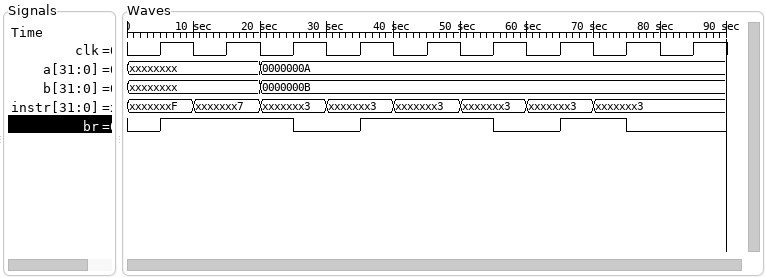
\includegraphics[scale=0.5]{diagrams/wave/branchtest.png}}
\caption[Κυματομορφή - Μονάδα Διαχείρισης Διακλαδώσεων]{Κυματομορφή λειτουργιών της μονάδας Διαχείρισης Διακλαδώσεων}
\end{figure}
\begin{description}
\item[Χρονική στιγμή 0] \hfill \newline
Προετοιμασία του σήματος εισόδου διανύσματος εντολής \texttt{jal}, με αδιάφορη τιμή x στα bit που δεν επηρεάζουν την λειτουργία της μονάδας.
\item[Χρονική στιγμή 5] \hfill \newline
Αποτέλεσμα απόφασης διακλάδωσης.
Το σήμα ενεργοποίησης διακλάδωσης παίρνει την τιμή \texttt{1}, ανεξαρτήτως των τιμών των εισόδων δεδομένων προς σύγκριση \texttt{A} και \texttt{B}.
\item[Χρονικές στιγμές 10, 15] \hfill \newline
Προετοιμασία του σήματος εισόδου διανύσματος εντολής \texttt{jalr}, με αδιάφορη τιμή x στα bit που δεν επηρεάζουν την λειτουργία της μονάδας, έχοντας ίδιο αποτέλεσμα με το παραπάνω.
\item[Χρονική στιγμή 20] \hfill \newline
Ανάθεση τιμών \texttt{0x0000000A} και \texttt{0x0000000B} στις εισόδους προς σύγκριση \texttt{A} και \texttt{B} αντίστοιχα.
Προετοιμασία του σήματος εισόδου διανύσματος εντολής \texttt{beq}, με αδιάφορη τιμή x στα bit που δεν επηρεάζουν την λειτουργία της μονάδας.
\item[Χρονική στιγμή 25] \hfill \newline
Αποτέλεσμα απόφασης διακλάδωσης με βάση την σύγκριση των εισόδων \texttt{A} και \texttt{B}.
Το σήμα ενεργοποίησης διακλάδωσης παίρνει την τιμή \texttt{0}.
\item[Χρονικές στιγμές 30, 35, 40, 45, 50, 55, 60, 65, 70, 75] \hfill \newline
Διαδοχικές αλλαγές του σήματος εισόδου διανύσματος εντολής, έτσι ώστε να ελεγχθεί η λειτουργία όλων των εντολών διακλάδωσης, καθώς και τα αποτελέσματά τους.
Το διάνυσμα μεταβάλλεται έτσι ώστε να κωδικοποιεί τις εντολές \texttt{bne}, \texttt{blt}, \texttt{bge}, \texttt{bltu}, \texttt{bgeu}, με αδιάφορη τιμή x στα bit που δεν επηρεάζουν την λειτουργία της μονάδας.
Τα αποτελέσματα απόφασης διακλάδωσης της κάθε μίας από αυτές τις εντολές εμφανίζονται στην τιμή του σήματος ενεργοποίησης διακλάδωσης, με τις τιμές \texttt{1} και \texttt{0} για εκτέλεση της διακλάδωσης ή όχι αντίστοιχα.
\end{description}
\newpage
\subsection{Μονάδα Διαχείρισης Κινδύνων}
Η μονάδα διαχείρισης κινδύνων δεν θα μπορούσε να εξομοιώσει τις λειτουργίες της ως αυτοτελής μονάδα.
Οι λειτουργίες της παρουσιάζονται παρακάτω, ταυτόχρονα με τις ολοκληρωμένες κυματομορφές του επεξεργαστή κατά την εκτέλεση ενός ενδεικτικού προγράμματος.

Η λειτουργία της και ειδικότερα ο χρονισμός των σημάτων εξόδου της μονάδας διαχείρισης κινδύνων βασίζεται στα στάδια διασωλήνωσης του συγκερκιμένου μοντέλου επεξεργαστή καθώς και στην καθυστέρηση της ανάγνωσης της μνήμης εντολών κατά έναν κύκλο.
Το σήμα ενεργοποίησης κινδύνου της μονάδας διαχείρισης κινδύνων συνδέεται άρρηκτα με τον μετρητή προγράμματος που διευθυνσιοδοτεί την μνήμη εντολών και με την λειτουργία της μνήμης εντολών.
Το σήμα εξόδου εντολής προς εκτέλεση και ο χρόνος που παραμένει αμετάβλητο βασίζεται στην δομή και το βάθος της διασωλήνωσης του μοντέλου του επεξεργαστή, καθώς και την διαφορά μεταξύ των κύκλων που εμφανίστηκε ο κίνδυνος δεδομένων.

\subsection{Μοντέλο Επεξεργαστή - Εκτέλεση Προγράμματος}
Για τις ανάγκες επίδειξης βασικής λειτουργικότητας του μοντέλου επεξεργαστή έχει συνταχθεί και μεταφραστεί ένα απλό πρόγραμμα Assembly, αξιοποιώντας τον υλοποιημένο Assembler.
Παρουσιάζονται οι εντολές του προγράμματος, καθώς και οι δυαδικές τους κωδικοποιήσεις, οι οποίες κατά την εκτέλεση αναγιγνώσκονται από την μνήμη εντολών.

\begin{table}[H]
    \centering
    \begin{tabular}{|c|c|}
    \hline
    \cellcolor{lgray} \textbf{Πρόγραμμα σε Assembly} & \cellcolor{lgray} \textbf{Περιεχόμενο Μνήμης Εντολών\footnotemark} \\\hline
    \lstinputlisting[language=C]{../prog.rva} & \lstinputlisting[language=C]{../instr.mem} \\\hline
    \end{tabular}
    \caption[Απλή Μετάφραση Προγράμματος]{\label{tab:widgets}Ένα απλό παράδειγμα μετάφρασης προγράμματος και αποθήκευσής του στην μνήμη εντολών}
\end{table}
\footnotetext{Η αποθήκευση των κωδικοποίησεων των εντολών στην μνήμη εντολών γίνεται με Little Endian τρόπο, ενώ στις κυματομορφές εμφανίζονται με Big Endian τρόπο.}

Στην τρέχουσα παραμετροποίηση, το μοντέλο επεξεργαστή είναι ορισμένο στο μέγεθος εντέλου 32-bit, άρα με υποστήριξη αρχιτεκτονικής συνόλου εντολών RV32I.
Το παραπάνω πρόγραμμα θα μπορούσε να εκτελεστεί και στο μοντέλο επεξεργαστή με παραμετροποίηση για υποστήριξη RV64I.

\newpage
Παράδειγμα εκτέλεσης βασικού προγράμματος:
\begin{figure}[H]
\centering
\renewcommand{\figurename}{Κυματομορφή} 
\makebox[\textwidth][c]{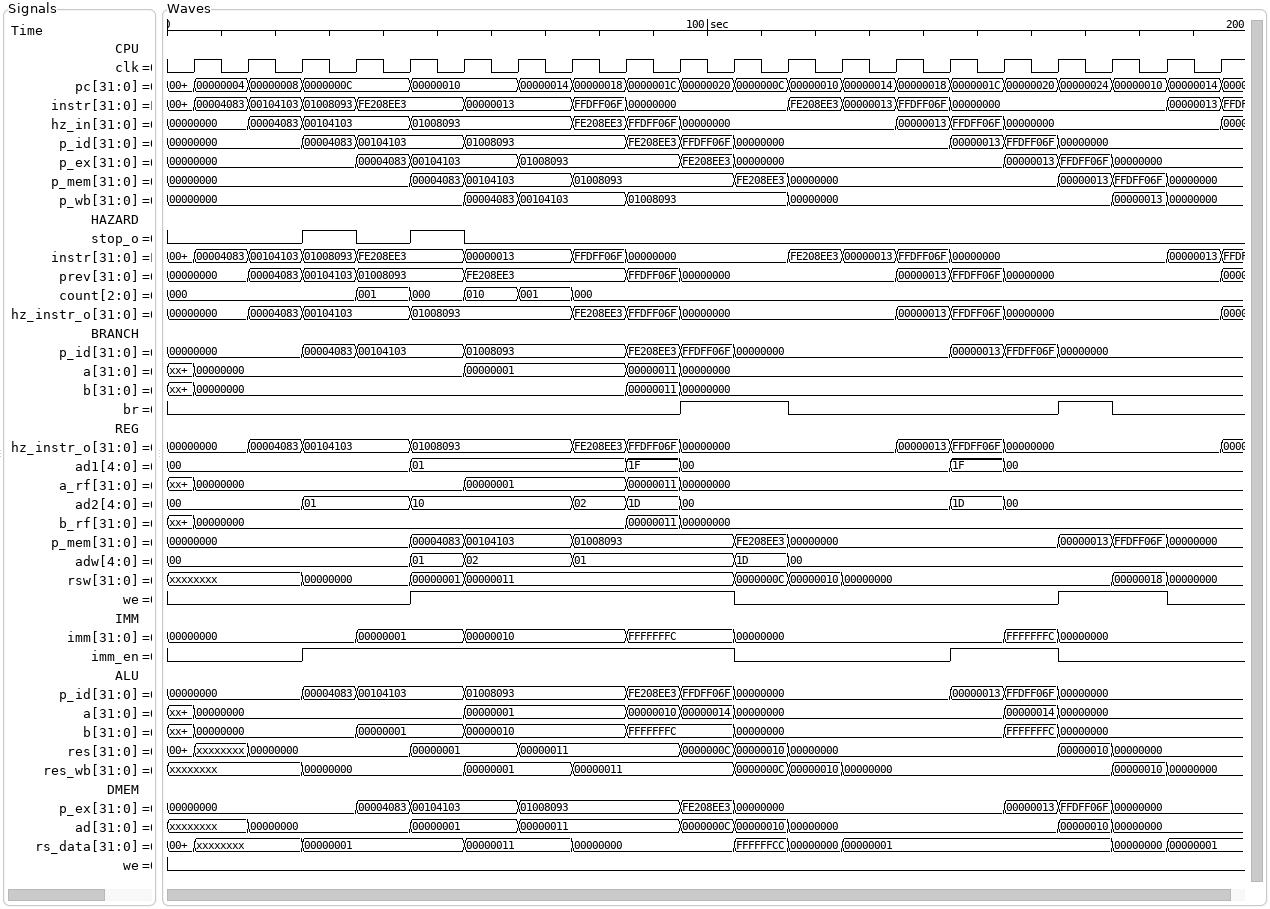
\includegraphics[scale=0.37]{diagrams/wave/cputest.png}}
\caption[Κυματομορφή - Παράδειγμα Εκτέλεσης Προγράμματος]{Κυματομορφή παραδείγματος εκτέλεσης προγράμματος στον επεξεργαστή}
\end{figure}

\begin{itemize}
    \item Το πρόγραμμα έχει κίνδυνο δεδομένου μεταξύ των εντολών μεταξύ των γραμμών 1 και 4, 2 και 5.
    Το πρόβλημα παρουσιάζεται με την ανάγνωση μετά την εγγραφή των καταχωρητών \texttt{x1}, \texttt{x2} αντίστοιχα.
    Παρατηρείται στα σήματα των καταχωρητών διασωλήνωσης η καθυστέρηση που δημιουργείται στην ανάθεση εντολών στα επόμενα στάδια διασωλήνωσης για 2 ή 3 κύκλους, για την αντιμετώπιση του κινδύνου.
    \item Παρατηρείται επίσης η εκκαθάριση των καταχωρητών της διασωλήνωσης για την αποφυγή εκτέλεσης του λάθος μέρους του προγράμματος μετά από την διακλάδωση.
    Τα στάδια που εκκαθαρίζονται είναι αρχικά τα στάδια ID και EX, και σε δεύτερο χρόνο το στάδιο MEM / WB.
    Με αυτόν τον τρόπο εξασφαλίζεται ότι η εντολή όπου λανθασμένα στάλθηκε προς εκτέλεση, δεν θα έχει επιρροή πέραν της ανάγνωσης καταχωρητών, πράγμα το οποίο δεν αλλάζει την κατάσταση του επεξεργαστή.
    Με την καθυστέρηση της εκκαθάρισης του σταδίου MEM / WB δίνεται ο απαραίτητος κύκλος στην προηγούμενη εντολή να εκτελέσει τις λειτουργίες αυτού του σταδίου.
    Η υλοποιημένη συμπεριφορά είναι συμβατή με τις προδιαγραφές, δηλαδή δεν υπάρχει παράθυρο εκτέλεσης εντολής καθυστερημένης διακλάδωσης.
    Επίσης, σε περίπτωση που αποφασιστεί να μην εκτελεστεί η διακλάδωση, δεν γίνεται εκκαθάριση των καταχωρητών και η εκτέλεση συνεχίζεται χωρίς κάποια καθυστέρηση για αναπροσαρμογή των καταχωρητών της διασωλήνωσης.
\end{itemize}



\section{ΜΕΛΛΟΝΤΙΚΕΣ ΒΕΛΤΙΣΤΟΠΟΙΗΣΕΙΣ}

Οι υλοποιήσεις που έχουν αναπτυχθεί στην διπλωματική εργασία είναι χρήσιμες για εκπαιδευτικούς σκοπούς όπως: 
\begin{itemize}
    \item Εξομοίωση του βασικού υποσυνόλου εντολών RISC-V RV32I.
    \item Παράδειγμα υλοποίησης ενός λειτουργικού και συμβατού με προδιαγραφές Assembler.
    \item Παρουσίαση των λειτουργιών ενός διασωληνωμένου επεξεργαστή σε επίπεδο εσωτερικών σημάτων.
    \item Ο συνδυασμός όλων των παραπάνω ως ένα ολοκληρωμένο λειτουργικό μοντέλο.
\end{itemize}

Η συγκεκριμένη διπλωματική εργασία ορίζει ένα βασικό θεμέλιο για την ανάπτυξη και ιδανικά την υλοποίηση ενός λειτουργικού μικροεπεξεργαστή.
Σε κάθε περίπτωση, υπάρχουν πολλές πτυχές της οι οποίες δύνανται να αναπτυχθούν περαιτέρω στο μέλλον, προσεγγίζοντας έναν πραγματικό μικροεπεξεργαστή.

\subsection{Υλοποίηση Επεκτάσεων}
Η αρχιτεκτονική συνόλου εντολών RISC-V ορίζει προαιρετικά υποσύνολα εντολών.
Θα μπορούσαν να αναπτυχθούν σε επίπεδο εξομοίωσης και να ενσωματωθούν στο συγκεκριμένο μοντέλο επεξεργαστή.

Ο Assembler επίσης είναι σχεδιασμένος με βάση την εύκολη επεκτασιμότητα, συνεπώς θα μπορούσε να χρησιμοποιηθεί για την παραγωγή συμβατών εκτελέσιμων με τον περαιτέρω ανεπτυγμένο επεξεργαστή.
Επεκτείνοντας παράλληλα τον επεξεργαστή και τον Assembler, δεν χρειάζεται να γίνει αλλαγή του τρόπου αποσφαλμάτωσης και ανάπτυξης που ακολουθήθηκε μέχρι στιγμής.

\subsection{Μικροαρχιτεκτονικές Βελτιώσεις}
Πολλοί υλοποιημένοι επεξεργαστές RISC-V αξιοποιούν τεχνικές όπως η out-of-order εκτέλεση εντολών και πολυπύρηνες μικροαρχιτεκτονικές.
Το μοντέλο προς το παρόν ορίζει έναν μονοπύρηνο in-order επεξεργαστή, η σχεδίασή του ωστόσο δεν περιορίζει την επέκταση των δυνατοτήτων του για ενσωμάτωση νέων σχεδιαστικών τεχνικών.

Πιο συγκεκριμένα, το στάδιο αντιμετώπισης Hazard που έχει προστεθεί στην κλασσική RISC διασωλήνωση, θα μπορούσε να χαρακτηριστεί ως μια πρώιμη μονάδα Instruction Issuing και Memory Ordering.
Μπορούν να υλοποιηθούν σχεδιαστικές τεχνικές όπως:
\begin{itemize}
    \item Instruction window για υποστήριξη out-of-order εκτέλεσης εντολών
    \item Register renaming για την γρηγορότερη διαχείριση των κινδύνων δεδομένων και εκτέλεση των προγραμμάτων
    \item Branch prediction για πρόβλεψη των αποφάσεων διακλαδώσεων
\end{itemize}

\subsection{Υλοποίηση σε Υλικό}
Έχει ήδη γίνει μια ενδεικτική σύνθεση των βασικών λειτουργικών μονάδων του επεξεργαστή σε FPGA, χωρίς να είναι ο κύριος στόχος αυτής της διπλωματικής εργασίας.
Φυσικά, μια περιγραφή υλικού γίνεται με σκοπό την πρακτική, λειτουργική υλοποίησή της.

Η ανάπτυξη ωστόσο ενός ολοκληρωμένου μικροεπεξεργαστή απέχει πολύ από μια διαδικασία εξομοίωσης και θεωρητικής υλοποίησης.
Αποτελεί πολύπλοκο, σύνθετο και χρονοβόρο εγχείρημα, που απαιτεί εξειδικευμένο εξοπλισμό, ανθρώπινο δυναμικό (πέραν του ενός ατόμου) τόσο για την σχεδίαση όσο και για την επιβεβαίωση της λειτουργικότητας της τελικής υλοποιημένης σύνθεσης υλικού.

\subsection{Υλοποίηση Βασικού Compiler}
Συμπληρωματικά με την λειτουργική υλοποίηση του μικροεπεξεργαστή, θα μπορούσε να αναπτυχθεί ένας C Compiler για την διευκόλυνση εκτέλεσης στατικών προγραμμάτων αρχικά, με τελικό στόχο την εκτέλεση ενός λειτουργικού συστήματος στον υλοποιημένο πλέον μικροεπεξεργαστή.

\subsection{Υποστήριξη συσκευών}
Φυσική απόρροια των ρεαλιστικών λειτουργικών υλοποιήσεων υλικού και της επιτυχούς εκτέλεσης ενός λειτουργικού συστήματος είναι η υποστήριξη διασύνδεσης συσκευών στο πλέον χρήσιμο σύστημα, μέρος του οποίου θα αποτελεί ο μικροεπεξεργαστής.
Το τελικό σύστημα θα μπορούσε να είναι ένας λειτουργικός μικροελεγκτής, ή ακόμα και μια πρώιμη μονάδα κεντρικής επεξεργασίας ενός ολοκληρωμένου υπολογιστικού συστήματος.

\section{ΠΑΡΑΡΤΗΜΑ - ΥΛΟΠΟΙΗΣΕΙΣ}
Όλες οι υλοποιήσεις βρίσκονται εδώ: \href{https://github.com/laskarelias/upatras-riscv}{https://github.com/laskarelias/upatras-riscv}
\subsection{Περιγραφή Υλικού - Verilog}
Ακολουθεί η περιγραφή υλικού κάθε μίας λειτουργικής μονάδας και του μοντέλου του επεξεργαστή, σε γλώσσα Verilog.
\subsubsection{Περιγραφή Μονάδας Μνήμης - mem.v}
\lstinputlisting[language=Verilog]{../mem.v}

\subsubsection{Περιγραφή Αριθμητικής - Λογικής Μονάδας - alu.v}
\lstinputlisting[language=Verilog]{../alu.v}

\subsubsection{Περιγραφή Αρχείου Καταχωρητών - regfile.v}
\lstinputlisting[language=Verilog]{../regfile.v}

\subsubsection{Περιγραφή Μονάδας Διαχείρισης Άμεσων Δεδομένων - immgen.v}
\lstinputlisting[language=Verilog]{../immgen.v}

\subsubsection{Περιγραφή Μονάδας Διαχείρισης Διακλαδώσεων - branch.v}
\lstinputlisting[language=Verilog]{../branch.v}
\newpage
\subsubsection{Περιγραφή Μονάδας Διαχείρισης Κινδύνων - hazard.v}
\lstinputlisting[language=Verilog]{../hazard.v}

\subsection{Εξομοίωση Υλικού και Testbench}
Ακολουθεί η περιγραφή των αρχείων εξομοίωσης των λειτουργικών μονάδων, σε γλώσσα Verilog.
\subsubsection{Testbench Μονάδας Μνήμης - memtest.v}
\lstinputlisting[language=Verilog]{../tests/memtest.v}
\newpage
\subsubsection{Testbench Αριθμητικής - Λογικής Μονάδας - alutest.v}
\lstinputlisting[language=Verilog]{../tests/alutest.v}

\subsubsection{Testbench Αρχείου Καταχωρητών - regtest.v}
\lstinputlisting[language=Verilog]{../tests/regtest.v}

\subsubsection{Testbench Μονάδας Διαχείρισης Άμεσων Δεδομένων - immtest.v}
\lstinputlisting[language=Verilog]{../tests/immtest.v}

\subsubsection{Testbench Μονάδας Διαχείρισης Διακλαδώσεων - branchtest.v}
\lstinputlisting[language=Verilog]{../tests/branchtest.v}

\newpage
\subsubsection{Testbench Μοντέλου Επεξεργαστή - tb.v}
\lstinputlisting[language=Verilog]{../tb.v}

\subsection{Αποτέλεσμα σύνθεσης}
Ακολουθούν τα αξιόλογα μέρη της εξόδου του εργαλείου Xilinx ISE κατά την διαδικασία της σύνθεσης των περιγραφών υλικού.
\lstinputlisting[language=C]{../tests/synthesis.txt}

\subsection{Κώδικας Assembler - Flex, Bison, C}
Ακολουθεί ο πηγαίος κώδικας σε Flex, Bison, C του προγράμματος του Assembler.
\subsubsection{Λεξικό Preprocessor - preproc.l}
\lstinputlisting[language=C]{../asm/preproc.l}

\subsubsection{Γραμματική Preprocessor - preproc.y}
\lstinputlisting[language=C]{../asm/preproc.y}

\subsubsection{Λεξικό Assembler - asm.l}
\lstinputlisting[language=C]{../asm/asm.l}

\subsubsection{Γραμματική Assembler - asm.y}
\lstinputlisting[language=C]{../asm/asm.y}

\subsubsection{Ορισμός symbol table - sym.h}
\lstinputlisting[language=C]{../asm/sym.h}

\subsubsection{Βασικό πρόγραμμα - main2.c}
\lstinputlisting[language=C]{../asm/main2.c}



\section{ΠΑΡΑΡΤΗΜΑ - ΕΡΓΑΛΕΙΑ}
Για την εκπόνηση της παραπάνω διπλωματικής εργασίας χρησιμοποιήθηκαν τα παρακάτω \textbf{εργαλεία}:
\begin{description}
    \item [vim] Επεξεργαστής κειμένου \newline
    Χρησιμοποιήθηκε κατά κόρον για την ανάπτυξη του πηγαίου κώδικα.
    \item [Visual Studio Code] Επεξεργαστής κειμένου - Περιβάλλον προγραμματισμού \newline
    Χρησιμοποιήθηκε κατά την συγγραφή του παρόντος τεχνικού κειμένου.
    \item [GTKWave] Πρόγραμμα προβολής κυματομορφών \newline
    Χρησιμοποιήθηκε κατά την εξομοίωση και αποσφαλμάτωση του μοντέλου του επεξεργαστή και για την παραγωγή των διαγραμμάτων κυματομορφών που βρίσκονται στο παρόν τεχνικό κείμενο.
    \item [Xilinx ISE] Περιβάλλον ανάπτυξης, εξομοίωσης και σύνθεσης υλικού \newline
    Χρησιμοποιήθηκε για την διαδικασία της σύνθεσης του μοντέλου του επεξεργαστή.
    \item [draw.io] Επεξεργαστής διαγραμμάτων \newline
    Χρησιμοποιήθηκε για την δημιουργία των αρχιτεκτονικών διαγραμμάτων και των διαγραμμάτων ροής του παρόντος τεχνικού κειμένου.
    \item [Github] Σύστημα ελέγχου εκδόσεων \newline
    Χρησιμοποιήθηκε για την ασφαλή αποθήκευση της προόδου της διπλωματικής εργασίας και επιπλέον για τον έλεγχο των διάφορων εκδόσεων που προέκυπταν κατά την ανάπτυξη και υλοποίησή της.
\end{description}
Χρησιμοποιήθηκαν επίσης οι παρακάτω \textbf{τεχνολογίες και γλώσσες}:
\begin{description}
    \item [Icarus Verilog] Γλώσσα περιγραφής υλικού \newline
    Χρησιμοποιήθηκε η γλώσσα περιγραφής υλικού Verilog για την περιγραφή των μονάδων του μοντέλου του επεξεργαστή και συγκεκριμένα ο εξομοιωτής Icarus Verilog.
    \item [Flex - Bison - C] Βιβλιοθήκες της C για ανάπτυξη parser \newline
    Χρησιμοποιήθηκαν για την ανάπτυξη του Assembler.
    \item [Latex (texlive) - pdflatex - bibtex] Γλώσσα markup  \newline
    Χρησιμοποιήθηκε για την συγγραφή του παρόντος τεχνικού κειμένου και πιο συγκεκριμένα, ο διερμηνευτής pdflatex.
    Για την διαχείριση της βιβλιογραφίας χρησιμοποιήθηκε το bibtex backend.
    \item [Makefile] Αυτοματοποίηση εκτελέσεων εντολών \newline
    Χρησιμοποιήθηκε για την αυτοματοποίηση εκτελέσεων εντολών για την μεταγλώττιση του Assembler, την εξομοίωση του μοντέλου του επεξεργαστή και την αυτόματη δημιουργία του εγγράφου κατά την διάρκεια της συγγραφής.
\end{description}
Φάνηκε χρήσιμη η παρακάτω \textbf{ιστοσελίδα}:
\begin{description}
    \item [venus] RISC-V Assembler (\href{https://www.kvakil.me/venus/}{https://www.kvakil.me/venus/} \cite{kvakil}) \newline
    Χρησιμοποιήθηκε πριν την ανάπτυξη του Assembler για παραγωγή απλών διανυσμάτων για εκτέλεση από τον επεξεργαστή και για την αποσφαλμάτωση και σύγκριση των αποτελεσμάτων του υλοποιημένου Assembler.
\end{description}

% \section{ΠΑΡΑΡΤΗΜΑ - ΠΙΝΑΚΕΣ ΣΥΝΟΛΟΥ ΕΝΤΟΛΩΝ RISC-V}
% ** όλες οι εντολές **
% ** ονόματα καταχωρητών **
% \section{ΠΑΡΑΡΤΗΜΑ - ΠΙΝΑΚΕΣ ΛΕΙΤΟΥΡΓΙΚΩΝ ΜΟΝΑΔΩΝ}
% ** ένας πίνακας i/o για κάθε module **
% \section{ΠΑΡΑΡΤΗΜΑ - ΔΙΑΓΡΑΜΜΑΤΑ ΜΙΚΡΟΑΡΧΙΤΕΚΤΟΝΙΚΗΣ}
% ** γενική αρχιτεκτονική **
% ** ενεργά module για κάθε τύπο εντολής **

\section{ΒΙΒΛΙΟΓΡΑΦΙΑ}
\printbibliography[heading=none]

\end{document}
